\chapter{Higgs Decay to Two Muons}\label{sec:hmumu}

\begin{figure}[h!]
\captionsetup[subfigure]{position=b}
\centering
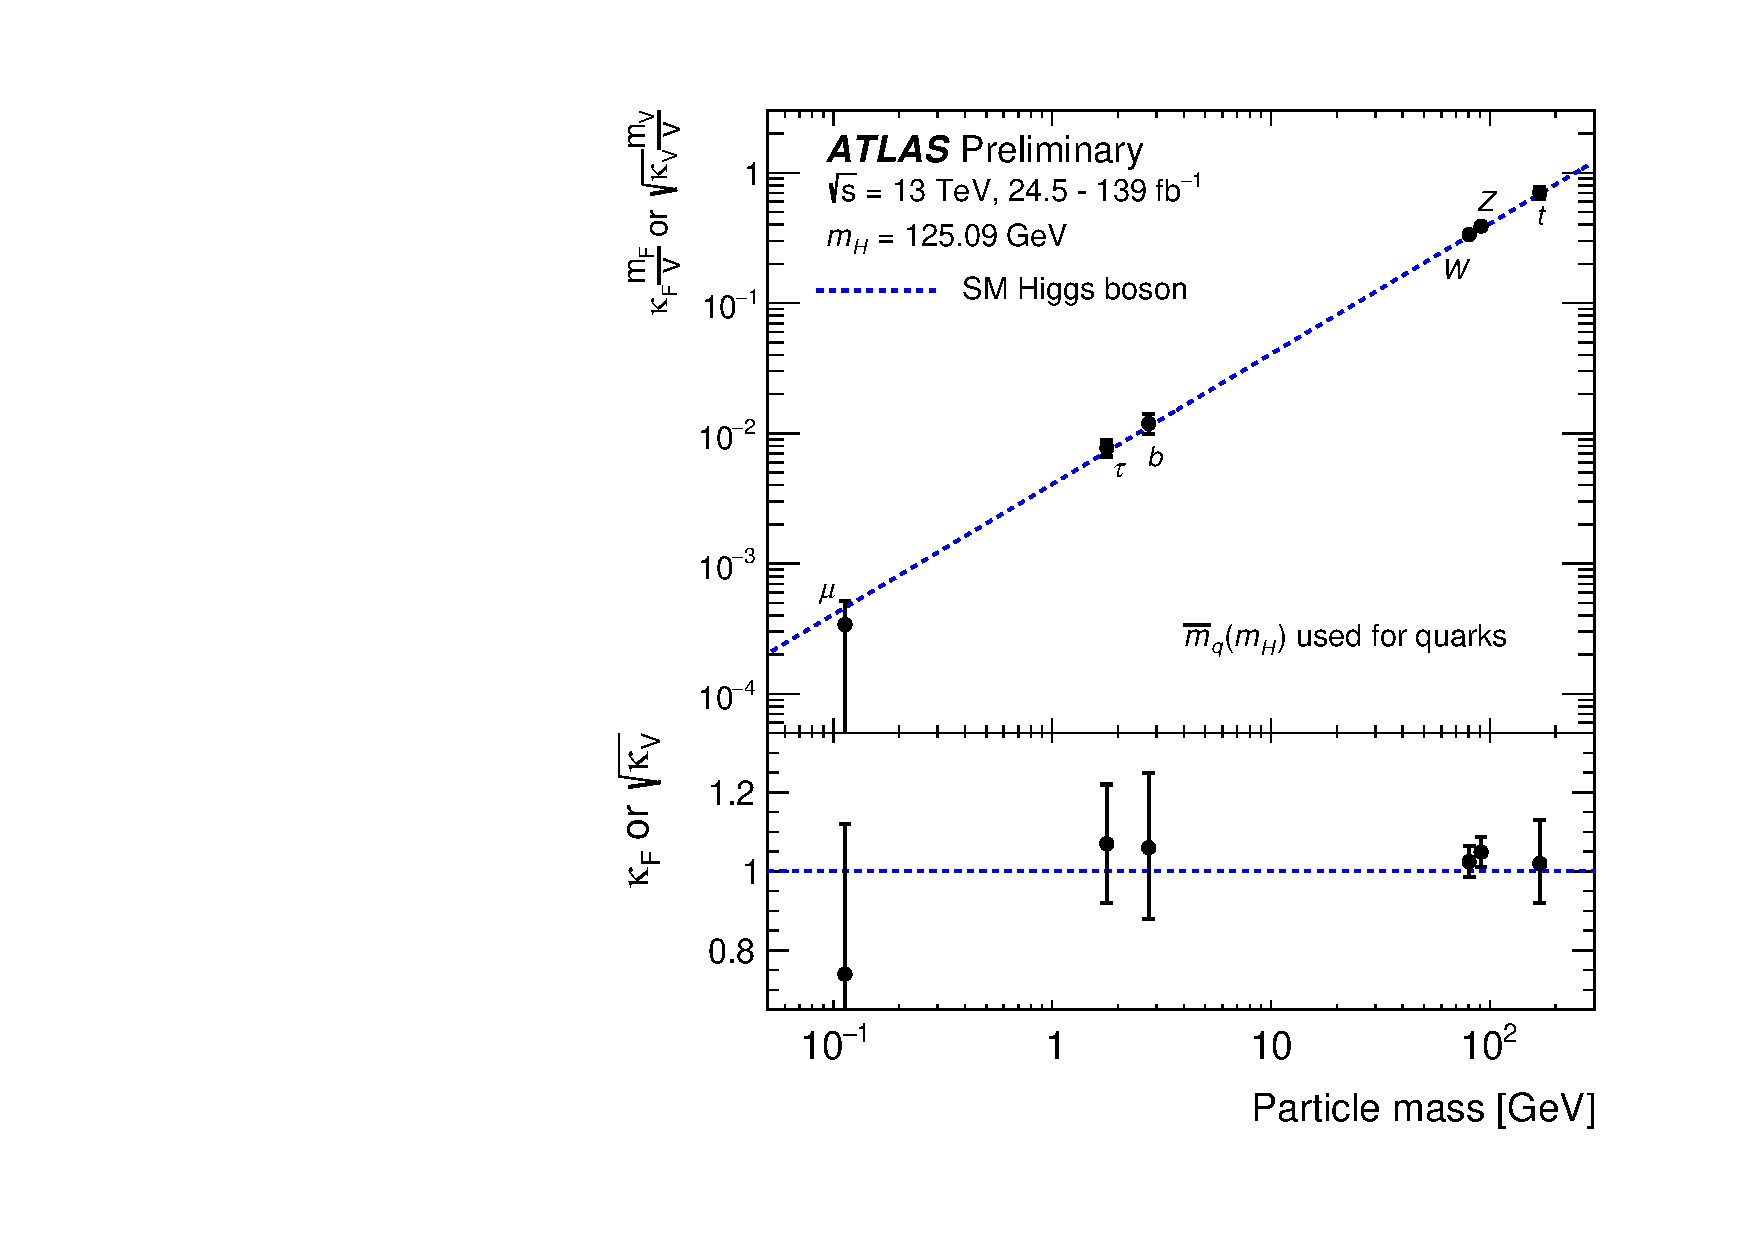
\includegraphics[width=0.5\textwidth]{figures/hmumu/massCouplingPlot.pdf}
\caption{Summary of ATLAS measurements of various fermion ($t$, $b$, $\tau$, and $\mu$) and gauge bosons. The plot shows the ``reduced coupling strength moderators'', where $\kappa$ is the deviation relative to the standard model prediction, compared to the particle's mass.
The SM prediction for both cases is also shown as a dotted line.
}
\label{fig:higgsMassCoupling}
\end{figure}

The joint observation of the Higgs boson by ATLAS \cite{atlashiggs} and CMS \cite{cmshiggs} in 2012 set the groundwork for the following study of this particle and its interactions.
One of the reasons that the Higgs boson is interesting is that the Englert-Brout-Higgs (BEH) mechanism generates mass terms for fermions through Yukawa couplings.
The most direct way to study these couplings is through the fermionic decay of the Higgs, described previously in Section \ref{sec:phenoHiggs}.
As the fermion branching ratios given Equation \ref{eqn:higgsDecayFermions} indicate, the Yukawa coupling is proportional to the fermion's mass squared.
Since the $H\to t\tbar$ decay is kinematically forbidden, the largest allowed branching fraction is to bottom quark pairs due to their large mass $m_b=4.2$~GeV. 
Despite this, the $Ht\tbar$ coupling can be measured through the ttH process described in Table \ref{tab:higgsProdDiagrams}.
The $Hb\bbar$ coupling was observed at the ATLAS experiment using the VH production channels. \cite{atlasHbb}
The next most massive fermion after the bottom quark is the tau lepton, with $m_\tau=1.8$~GeV, which has been studied by ATLAS \cite{atlasTauTau} and CMS \cite{cmsTauTau}.
% I don't want the thesis to be immediately out of date
Although the charm quark with comes next at $m_c=1.3$~GeV, the messy final state proves difficult to identify and study.
Searches for $H\to c\cbar$ remain insensitive even to $Hc\cbar$ couplings $\sim100$ times the standard model expectation.
This leaves the muon and the $H\mm$ coupling, where the muon's mass of $\m_\mu=0.1$~GeV results in a challengingly small branching fraction.
However unlike the case with the charm quark, the final state of two muons is easily identified.
The result is that the $H\mm$ is the third and most challenging Higgs Yukawa coupling that is feasible to study at ATLAS.

The $H\mm$ coupling is also unique, as both the $Hb\bbar$ and $H\tautau$ couplings are to third generation fermions.
This means that the \hmm measurement adds a valuable point to the global picture of Higgs couplings as illustrated in Figure \ref{fig:higgsMassCoupling}.
Measuring this coupling provides a test of the standard model, and also insight into the origin of the muon's mass.

Detecting the decays of Higgs to two muons is particularly challenging on two counts.
First, the Higgs branching fraction to muons is tiny ($2.18\times10^{-4}$).
Second, there is a large irreducible dimuon background from Drell-Yan and Diboson processes.
Together these evoke the idiomatic needle-in-a-haystack to describe the search for \hmm.
It is only with the enormous number of events collected by ATLAS during the Run 2 data taking campaign that became feasible to perform this search.

%%%%%%%%%%%%% VH #################3

Of particular interest in this thesis are Higgs boson produced through the VH production mechanisms.
These events offer both a chance to look at a new, unobserved phase space, as well as a contribution to the overall \hmm sensitivity.
The events where the vector boson decays leptonically are particularly useful.
The additional leptons in these events help to differentiate VH from the Drell-Yan background, and also provide kinematic information for further discrimination.

\begin{table}[htbp]
 \begin{center}
\begin{tabular}{l r r r r r}\toprule
   & $H\to\mu\mu$ & $H\to\mu\mu V\to\ell\ell$ \\
WH & 41.5 & 9.14 \\
ZH & 26.9 & 1.83 \\
\bottomrule\end{tabular}
 \end{center}
 \caption{Expected numbers of events from 139 fb$^{-1}$ $\sqrt{S}=13$ TeV data for WH and ZH. The first column shows the number of VH events times BR($H\to\mu\mu$), while the second column additionally multiplies by BR($V\to\ell\ell$) where $\ell$ is $e$ or $\mu$.}
\label{tab:vh-predict}
\end{table}

Studying VH/\hmm comes with additional challenges.
First is the tiny VH cross section leading to relatively few signal events.
Second is how to use the new information from the W/Z leptonic decay products to separate the background from diboson production processes (ZZ and WZ).
% Techniques to address challenge
Careful choices are made in the selection criteria targeted at VH production in order to capture as many VH/\hmm events as possible.
A multivariate analysis (MVA) discriminant is used to take advantage of the kinematic information from the W/Z decays.
Again careful steps must be taken in order to understand and limit the level of bias in the results that these techniques introduce, and avoid invalidating the final measurements.

\begin{figure}[htpb]
  \centering
    \centered{\begin{tikzpicture}
    \begin{feynman}
        \vertex (qa){\(\qbar\)};
        \vertex [below right=of qa] (p1);
        \vertex [below left=of p1] (qb){\(q'/q\)};
        \vertex [right=of p1] (p2);
        \vertex [above right=of p2] (h){\(H\)};
        \vertex [below right=of p2] (v){\(W/Z\)};
        \diagram* {
        (qb) --[fermion] (p1) --[fermion] (qa),
        (p1) --[boson,edge label=\(W/Z\)] (p2),
        (v) --[boson] (p2) --[scalar] (h),
        };
    \end{feynman}
    \end{tikzpicture}} 
  \caption{VH production originating from quarks}
    \label{fig:vh-prod}
\end{figure}

The VH production mechanisms, WH and ZH, shown in figure \ref{fig:vh-prod}, are the third and fourth leading Higgs boson production mechanisms at the LHC. The $\sqrt{S}=13$ TeV cross section of WH is 1.36 pb, and the cross section of ZH is 0.88 pb. The cross section, combined with the branching ratio of $H\to\mu\mu$ of $2.18\times10^{-4}$, result in the number of expected events per 139 fb$^{-1}$ shown in the first column of table \ref{tab:vh-predict}. In addition to the quark originating ZH shown in figure \ref{fig:vh-prod}, gluon originating ZH (via quark loop and contributing $\approx10\%$) is also considered.


\begin{figure}[h!]
\captionsetup[subfigure]{position=b}
\centering
\subfloat[][]{{
    \feynmandiagram [small,baseline=(v.base),horizontal=a to v] {a[particle=\(W^\pm\)] --[boson] v --[fermion] b[particle=\(\ell^\pm\)], c[particle=\(\nu\)] --[fermion] v,};
}}
\hspace{3em}
\subfloat[][]{{
    \feynmandiagram [small,baseline=(v.base),horizontal=a to v] {a[particle=\(Z\)] --[boson] v --[fermion] b[particle=\(\ell^+\)], c[particle=\(\ell^-\)] --[fermion] v,};
}}
  \caption{Leptonic decays of the \W (a) and \Z (b) bosons.}
  \label{fig:vh-decay}
\end{figure}

Five categories are used for the search.
Two are based on a four-lepton selection designed to capture ZH events, and three are based on a three-lepton selection optimized for WH events.
These consider leptonic ZH events with $\mu\mu\mu\mu$ or $ee\mu\mu$ final states, and leptonic WH events with $\mu\nu\mu\mu$ or $e\nu\mu\mu$.
In the case of leptonic decays of the \W, only the charged lepton is reconstructed, while some inference about the neutrino may be obtained from the missing transverse energy.
The delimitation within a selection is based on the MVA discriminant, resulting in categories with high signal purity and low signal purity.
The final search is performed in the dimuon invariant-mass spectrum across five categories.

This chapter describes the search for \hmm using the VH production channels with the full Run 2 dataset collected by ATLAS.
Section \ref{sec:hmmEvSel} describes the selection of data used for the search, followed by Section \ref{sec:hmmBdt} that describes the MVA based categorization.
Sections \ref{sec:hmmSig} and \ref{sec:hmmBkg} present the signal and background models, respectively.
Next Section \ref{sec:hmmSyst} discusses the systematic uncertainties used in the result.
Section \ref{sec:hmmStat} details the statistical analysis of the data.
Finally Section \ref{sec:hmmResults} presents the results of the analysis.

\section{Data and Event Selection}\label{sec:hmmEvSel}

The search for \hmm is concerned with events containing at least two muons.
This section details the event selection, data, and simulation used in the analysis.

\subsection{Event Selection}\label{sec:hmmEv}

All data events are required to pass several criteria before they are considered for analysis.
Events are considered only if they were recorded while the ATLAS detector was in full operation.
The events meeting this requirement comprise the Good Run List, as summarized in Section \ref{sec:physData}.

Only a small fraction of the many events observed by ATLAS are useful to study. 
The trigger system decides on an event-by-event basis whether to record an event. 
Since \hmm events have muons in their final state, the analysis uses a trigger selection that requires at least one high-\pt muon.
The \pt threshold varies based on the year of data taking, depending on the trigger system's configuration.
In 2015 the minimum threshold was $\pt>20$~GeV, while in other years, it was $\pt>26$~GeV.
Muons with a \pt below 50~GeV are required to have isolated tracks in the ID to reduce the background event rate.
The efficiency of the trigger requirement is $\approx90\%$.

% Object selection
After passing the trigger requirement, the physics objects that comprise the event are tabulated.
The most important objects for leptonic VH \hmm are muons and electrons, but jets and \met are also used to reduce the background.
The definitions of the objects make use of identification and isolation requirements defined in Section \ref{sec:physObjects}.

The muons considered in an event meet the requirements listed in Table \ref{tab:hmmMuonObjSel}.
These can come from the Higgs decay, as well as the leptonic \W and \Z decays.
These are selected to be relatively inclusive due to the rarity of \hmm decays.
All four types of muons are used: CB, CT, ST, SA.
A particularly low \pt threshold of 6~GeV is selected with the four-muon ZH events in mind since one of the four muons often has a low \pt.

% Muons
\begin{table}[H]
    \begin{center}
        \begin{tabular}{ll}
            \toprule
            Type            &CB, CT, ST, SA\\
            Identification  &Loose \\
            Isolation       &FixedCutPflowLoose\\
            $\pt$           &$\pt > 6$~GeV\\
            $\eta$          &$|\eta| < 2.7$\\
            \multirow{2}{*}{Impact parameters}   &$|d_0^{\mathrm{BL}}/\sigma_{d_0^{\mathrm{BL}}}| < 3$\\
            &$|z_0^{\mathrm{PV}}\cdot \sin{\theta}| < 0.5$~mm\\
            \bottomrule
        \end{tabular}
        \caption{Muon selection criteria.}
        \label{tab:hmmMuonObjSel}
    \end{center}
\end{table}

The electrons are considered next, as these are produced by leptonic \W and \Z decays.
With a similar motivation to the muons, this selection is relatively lenient to maximize the selection's efficiency.
Several criteria are included to retain as many prompt electrons as possible while reducing the inclusion of fake electrons.
These are listed in Table \ref{tab:hmmEleObjSel}.

\begin{table}[H]
    \begin{center}
    %\footnotesize
        \begin{tabular}{ll}
            \toprule
            Identification    &Medium LH\\
            Isolation        &FCLoose\\
            $\pt$            &$\pt > 7$~GeV\\
            $\eta$            & $|\eta|<1.37$ or $1.52<|\eta|<2.47$ \\
            Quality            &Not "BADCLUSELECTRON"\\
            \multirow{2}{*}{Impact Parameters}    & $|d_0^{\mathrm{BL}}\ \mathrm{significance}|<5$ \\
            &$|z_0^{\mathrm{PV}} \cdot \sin{\theta}| < 0.5$~mm\\
            \bottomrule
        \end{tabular}
        \caption{Electron selection criteria.}
        \label{tab:hmmEleObjSel}
    \end{center}
\end{table}

Jets are reconstructed in order to remove background events from the VH selection.
The VH leptonic events are expected to produce small jet multiplicities.
Furthermore, jets are used to reduce the presence of ttH events in the selection, by vetoing events that a b-jet.
The criteria for jet selection are given in Table \ref{tab:hmmJetObjSel}.

\begin{table}[H]
    \begin{center}
    %\footnotesize
    \begin{tabular}{ll}
        \toprule
        Algorithm        &AntiKt R=0.4 PFlow\\
        $\eta$            &$|\eta| < 4.5$    \\
        $\pt$            &$\pt > 25$~GeV for $|\eta| < 2.4$, $\pt > 30$~GeV for $2.4 < |\eta| < 4.5$ \\
        % JVT                & $\mathrm{JVT} > 0.59$ for $|\eta| < 2.4$ and 20~GeV$ < \pt < $120~GeV, $\mathrm{JVT} > 0.11$ for $2.4 < |\eta| < 2.5$ and 20~GeV$ < \pt < $120~GeV\\
        \bottomrule
    \end{tabular}
    \caption{Jet selection criteria. Additionally, a combination of track-based variables are used suppress jets from other collisions in the same bunch crossing, called jet-vertex-tagger.\cite{ATLAS-CONF-2014-018}}
    \label{tab:hmmJetObjSel}
    \end{center}
\end{table}

Finally, the missing transverse momentum, \met, is calculated for the event.
The \met is calculated from the \pt of all reconstructed muons, electrons, and tracks not identified with one of these.
This serves as a proxy for the undetected neutrino from leptonic \W decays.

\begin{table}[htp]
\begin{center}
\begin{tabular}{l l l l}
\toprule
Reject & Against & Condition \\
\midrule
\centered{Jet} & \centered{Electron} & \centered{$\Delta(e,\text{jet})R<0.2$} \\ 
\centered{Jet} & \centered{Muon} & \centered{$\Delta(\mu,\text{jet})R<0.2$} \\ 
\centered{Electron} & \centered{Electron} & \centered{lower \pt electron of shared track} \\ 
\centered{Electron} & \centered{Muon} & \centered{share track} \\ 
\centered{Electron} & \centered{Jet} & \centered{$0.2<\Delta(e,\text{jet})R<0.4$} \\ 
\centered{Muon} & \centered{Electron} & \centered{is calo-muon and shares track} \\ 
\centered{Muon} & \centered{Jet} & \centered{$0.2<\Delta(\mu,\text{jet})R<0.4$} \\
\bottomrule
\end{tabular}
\caption{Overlap removal criteria adopted for object selection, applied sequentially. The jet removal against muons is applied for jets satisfying $N_{Trk}(jet)<3$, or ($p_\mathrm{T}^{jet}/p_\mathrm{T}^{\mu}<2$ and $p_\mathrm{T}^{\mu}/\Sigma_{TrkPt}>0.7$)}
\label{tab:hmmOr}
\end{center}
\end{table}

An overlap removal scheme is applied to avoid treating the same detector signature as multiple objects when two objects are reconstructed in close proximity.
This scheme removes objects according to the priorities listed in Table \ref{tab:hmmOr}.

Once the objects within an event have been determined, the next step is to identify events with objects matching the final state of leptonic VH processes.
All events are required at least one oppositely-charged muon pair that can serve as a candidate for \hmm.
Two parallel selections are carried out: 3-lepton events are selected targeting the WH process, while 4-lepton events are selected targeting the ZH process.

In events with two exactly two muons, these are required to be oppositely charged. In events with more than two muons, later charge requirements are applied, as described in table \ref{tab:hmmEv}. The leading $p_T$ muon is required to have $p_T>27$ GeV. The sub-leading $p_T$ muon is required to have $p_T>8$ GeV. The threshold for the sub-leading muon is lowered compared to the ggF/VBF selection to increase the signal yield efficiency. This change, in conjunction with the lower $p_T$ threshold for all muons and the loosening of the opposite charge requirement, increases WH signal yield by 16.9\% and ZH signal yield by 63\%.

Two selections are used to target VH production: a \textbf{3-lepton} category that targets WH production where the W decays leptonically (electrons or muons), and a \textbf{4-lepton} category that targets ZH production where the Z decays leptonically (electrons or muons).
The overall signal efficiency of the WH event selection is 45\%.
The signal efficiency of the ZH event selection is 37\%.
Both of the efficiencies are calculated with respect to the \W/\Z bosons decaying into electrons or muons.

The leptonic VH production does not produce many b-jets, in contrast to the top backgrounds and ttH signal production.
A veto of events containing b-jets helps reduce these backgrounds and also enhances the purity of the signal selection.
Section \ref{sec:expJets} describes how b-jets are identified with several working points that specify the efficiency of identifying a b-jet.
The loosest working point, 85\%, is selected based on its reaction of the background.
Figure \ref{fig:hmmBveto} illustrates signal and background yields in a comparison between vetoes using the 60\% and 85\% working points.
The looser 85\% working point constitutes a stricter veto, and it is seen to reduce the background yields in both the 4-lepton and 3-lepton selections.
The signal yields are not substantially affected.


\begin{figure}[h!]
\captionsetup[subfigure]{position=b}
\centering
\subfloat[][]{{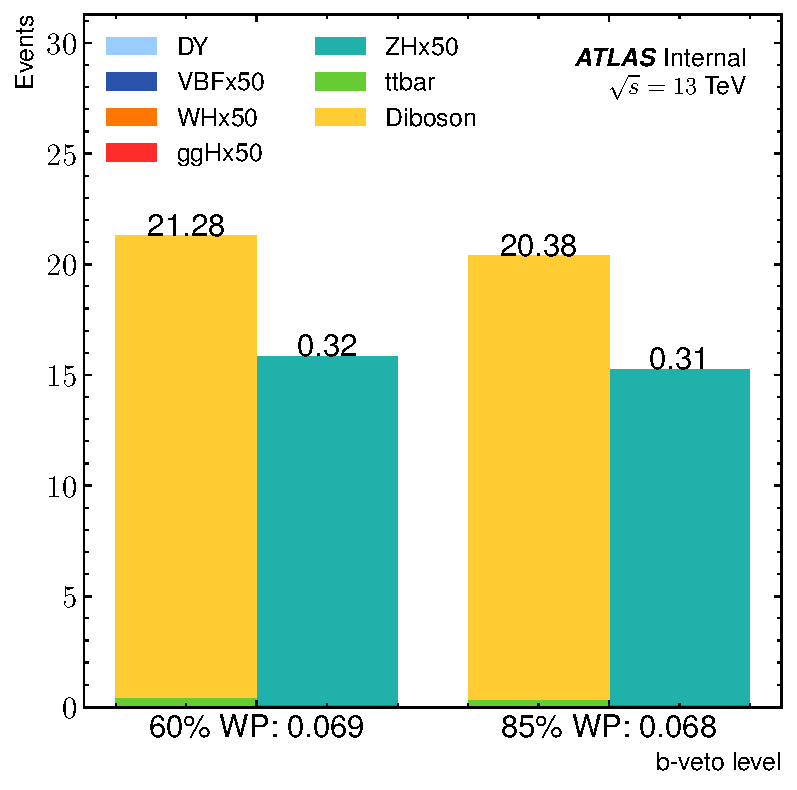
\includegraphics[width=0.5\textwidth]{figures/hmm/bveto/btag-4lep.pdf}}}
\subfloat[][]{{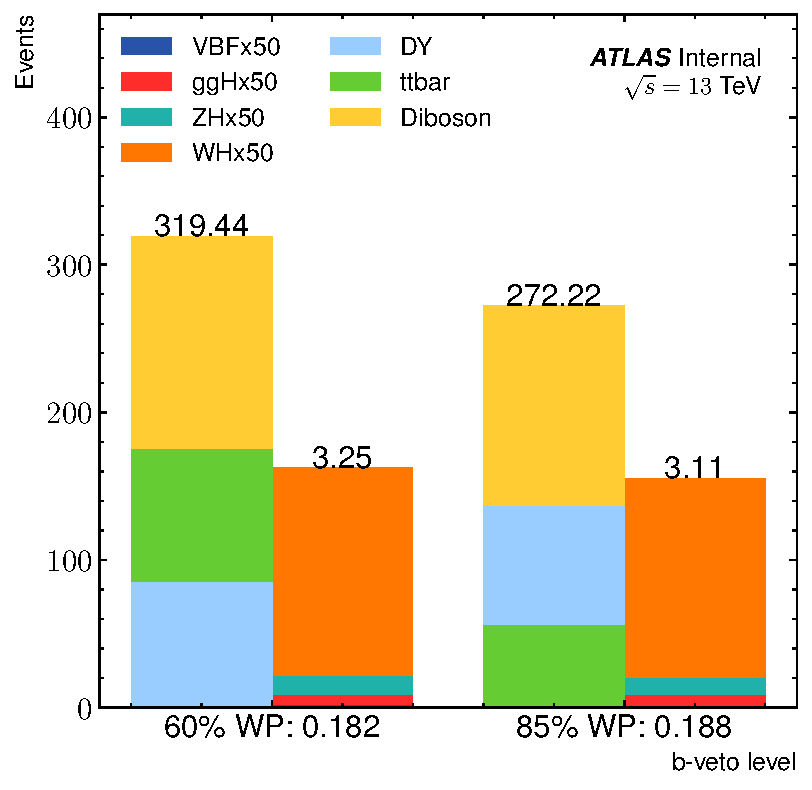
\includegraphics[width=0.5\textwidth]{figures/hmm/bveto/btag-3lep.pdf}}}
\caption{Illustration of the impact on signal and background yields of using different btag working points (WP) for the b-jet veto. This is shown for the 4-lepton selection (a) and 3-lepton selection (b). Each bar shown the number of simulated signal or background events passing the selection when using the WP marked on the x-axis. For both selections, using the looser 85\% WP reduces the background yields compared to the tighter 60\% WP. At the same time, the signal yield is relatively unchanged.}
\label{fig:hmmBveto}
\end{figure}

\begin{table}[ht!]
 \begin{center}
\begin{tabular}{c c  c}\toprule
Step & 4-lepton & 3-lepton \\\midrule
1 & \multicolumn{2}{c}{No 85\% WP btag jets (b-jet veto)}           \\\midrule
2 & At least 4 leptons                                & Exactly 3 leptons\\\midrule
3 & ($N_{\mu^+}>$0 and $N_{\mu^-}>$0)                 & ($N_{\mu^+}>$0 and $N_{\mu^-}>$0) \\\midrule
4 & A dimuon pair $\exists\in$ [110,160] GeV                    & A dimuon pair $\exists\in$ [110,160] GeV \\\midrule
\multirow{2}{*}{5} & ($N_{\mu^+}>$1 and $N_{\mu^-}>$1) or              & ($N_{\mu^+}>$1 or $N_{\mu^-}>$1) or \\
  & ($N_{e^-}>$0 and $N_{e^+}>$0)                    & ($N_{e^-}>$0 or $N_{e^+}>$0)  \\\midrule
6 & $\nexists$ two Z$\to\mu\mu$ candidates                        & $\nexists$ Z$\to\mu\mu$ candidate  \\\midrule
7 & Higgs candidate $\in$ [110,160] GeV                  & Higgs candidate $\in$ [110,160] GeV \\\midrule
\multirow{2}{*}{8} & Kinematic cuts 27/15/8/6 GeV $>p_T$                    & Kinematic cuts 27/10/15(10) GeV $>p_T$ \\
  &                                                        & for $e(\mu)$ \\
\bottomrule\end{tabular}
 \end{center}
 \caption{Cutflow for 4-lepton and 3-lepton selection. Lepton pairs are opposite charge.}
\label{tab:hmmEv}
\end{table}

The steps of the cutflow are shown in table \ref{tab:hmmEv}, which defines the 4-lepton and 3-lepton VH candidate categories.
This cutflow defines ``\Z candidates'' to be oppositely charged dimuon pairs an invariant-mass in $[80,105]$~GeV.
The selection of oppositely charged muons for the Higgs candidate, and of additional leptons for the \Z(\W) candidates is based on minimizing a $\chi^2$ calculation related to the invariant-mass (transverse-mass) of the candidates.
This is shown in equations \ref{eq:hmmWhPairing} and \ref{eq:hmmZhPairing}.
Here, for each candidate pairing, $\chi^{2,\text{cand}}$ is calculated from the Higgs candidate mass $M_H^\text{cand}$.
For 4-lepton events, the \Z candidate mass $M_Z^\text{cand}$ is used, and for 3-lepton events the transverse-mass of the W candidate lepton and $E_T^\text{miss}$, $M_T^\text{cand}$, is used.
Only pairings with oppositely charged muons are considered for $M_H^\text{cand}$, while all oppositely charged same flavor pairs are considered for $M_Z^\text{cand}$.
Leptons of both flavors and charges are considered for $M_T^\text{cand}$.
The pairing with the smallest $\chi^{2,\text{cand}}$ is selected.

\begin{equation}
  \label{eq:hmmWhPairing}
  \chi^{2,\text{cand}} = (M_H^\text{cand}-125\text{ GeV})^2/(3.0\text{ GeV})^2 + (M_T^\text{cand}-70\text{ GeV} )^2/(20\text{ GeV})^2
\end{equation}

\begin{equation}
  \label{eq:hmmZhPairing}
  \chi^{2,\text{cand}} = (M_H^\text{cand}-125\text{ GeV})^2/(3.0\text{ GeV})^2 + (M_Z^\text{cand}-91.1\text{ GeV} )^2/(3\text{ GeV})^2
\end{equation}

The $\chi^2$ pairing is used to improve the pairing efficiency.
Other pairing procedures were considered but were rejected based on their performance.
For example, in 4-muon events, selecting the highest $p_T$ opposite sign muon pair is 63.4\% less efficient than the $\chi^2$ pairing described above. 
Selecting the pair such that the \Z candidate is closest to the \Z mass is 8.7\% less efficient.

The cuts described in table \ref{tab:hmmEv} define two categories of events, 3-lepton and 4-lepton, which are referred to as inclusive categories in relation to the subsequent division into smaller categories.
The kinematic distributions of the leptons in these categories are illustrated in Section \ref{sec:hmmKine}.

\subsection{Simulation}\label{sec:hmmSim}

Simulated datasets play a central role in the search strategy.
All simulated datasets are scaled to match their corresponding cross-section.\cite{CERNYellowReport4}
First, the simulated background and signal datasets allow an exploration of the efficiency of various event selection criteria.
This eventually leads to the criteria listed in Table \ref{tab:hmmEv}.
Next, probability density distributions are constructed from simulated events that describe the probability to observe variables at a given value.
This is done both both for background and signal productions.
This allows the development of a multivariate discriminant function that separates signal and background events based on these variables.
% Simulated events are used at each step of this process: to determine the discriminant function with one set of simulated events and constrain the level of bias it may introduce with a second set of events.
% After this, an unrelated third set is used to estimate the rates of signal and background events, as a function of dimuon invariant mass, at different levels of discrimination.
The background rates as a function of \muu are used to measure systematic uncertainties and to validate the performance of several empirical background models.
The signal shape is used for these purposes as well, and most importantly, it provides the signal component in the hypothesis test performed on the observed data.
Finally, several theoretical and experimental variations on the signal shape are used to measure the impact of these uncertainties on the final result.

% Background ========================
The primary background production in the region of interest comes from Drell-Yan (DY), Diboson, and top production mechanisms described in section \ref{sec:phenoBkg}.
The dominant background mechanism, DY, primarily produces events with two leptons in the final state.
This is reduced through the requirement of more than two leptons in the event selection.
Processes involving $t\tbar$ and single-top production form a large background component as well.
Since the top quark always produces a bottom quark through decay, these backgrounds are mitigated by use of the b-jet veto in the event selection.
After this are diboson productions of $ZZ$ or $WZ$ with leptonic decays.
The diboson is topologically the most similar to the VH signal, making this the most challenging process to reject.
Diboson events are reduced with the help of a discriminant function based on several kinematic observables, but these events remain the dominant background after all selections are complete.

The DY simulations are generated with \sherpa 2.2.1 using the NNPDF3.0 PDF.
The DY \muu spectrum falls exponentially.
To generate sufficient numbers of high-mass events, these are simulated in ranges of $x$, where $x$ is the maximum of the mediator \pt and the scalar parton \pt sum, \httt.
These simulations are produced to NLO for diagrams, including fewer than three jets and LO for diagrams, including three or four jets.

The $t\tbar$ and single-top simulations are produced with \powheg v2 and the NNPDF3.0NLO PDF.
The mass of the top quark is set to $m_t=172.5$.
The $t\tbar$ cross section is calculated to NNLO using Top++2.0. \cite{Czakon:2011xx}
The leading order $t\tbar$ Feynman diagrams are shown in Figure \ref{fig:phenoTtbar}.
The cross-sections of single-top production channels are calculated to NNLL accuracy following the standard procedure. \cite{Kidonakis:2011wy, Kidonakis:2010ux}
The leading order single-top Feynman diagrams are shown in Figure \ref{fig:phenoSingleTop}.
Different simulations are generated for $s$-channel and $t$-channel production through the exchange of a \W boson. A sample is produced for single-top production in association with a \W as well.

The final background simulations are composed of the diboson processes $WZ$ and $ZZ$ with leptonic decays.
These are produced with \sherpa 2.2.1 (for quark decays) and \sherpa 2.2.2 (for fully leptonic decays) and the NNPDF3.0 PDF.
Some number of leptonic decays are needed in order to be interesting for the purpose of the analysis.
One set of simulations simulates $$ZZ$\to q\qbar\ll$ and $$WZ$\to q\qbar\ll$ events, while a second set simulates events with $\ll\ll$, $\ll\ell\nu$, and $\ll\nu\nu$ final states. \cite{ATL-PHYS-PUB-2017-005}
The purely leptonic $\ll\ll$ originates from two \Z decays.
This is the primary background in the 4-lepton categories and shares a very similar topology to ZH.
For completeness, the $ZZ$ decay to $\ll\nu\nu$ is simulated as well.
The production of $WZ$ $\ll\ell\nu$ is the primary background for several 3-lepton categories.
The leading order diboson Feynman diagrams are shown in Figure \ref{fig:phenoDiboson}.

% Signal simulations ========================
Signal simulations are produced based on the dominant Higgs production mechanisms listed in Table \ref{tab:higgsCrossSec}.
Most simulations are simulated with a Higgs mass set to 125~GeV using \powheg v2 and the PDF4LHC15 PDF. 
The exception is ttH, which is produced with \madgraph and the NNPDF3.0NLO PDF.
The precision ranges from NNLO in QCD for the ggF, to NLO for the VBF, VH, and ttH mechanisms.
The contribution of $gg\to ZH$ is simulated at LO.


\subsection{Kinematic Distributions}\label{sec:hmmKine}

The pre-cut categories defined in Section \ref{sec:hmmEv} are illustrated here with the aid of the simulated signal and background simulations.
The mass distributions are presented in Figure \ref{fig:hmmPrecutMassHists}.
These provide an illustration of the composition of the background and signal contributions to these categories, as well as the general agreement between data and simulation. 

\begin{figure}[h!]
\captionsetup[subfigure]{position=b}
\centering
\subfloat[][]{{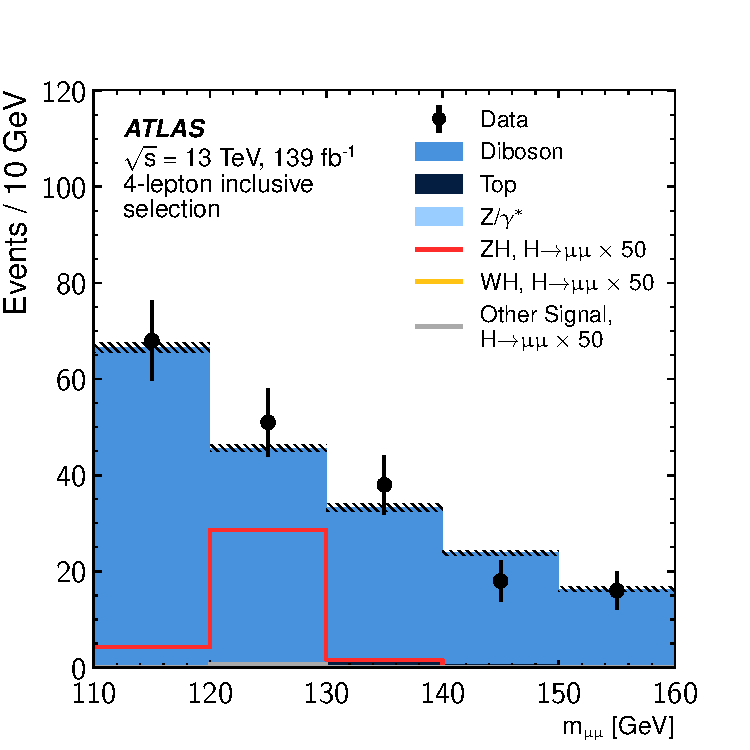
\includegraphics[width=0.5\textwidth]{figures/hmm/public/preCut/histo-4lep-muu.pdf}}}
\subfloat[][]{{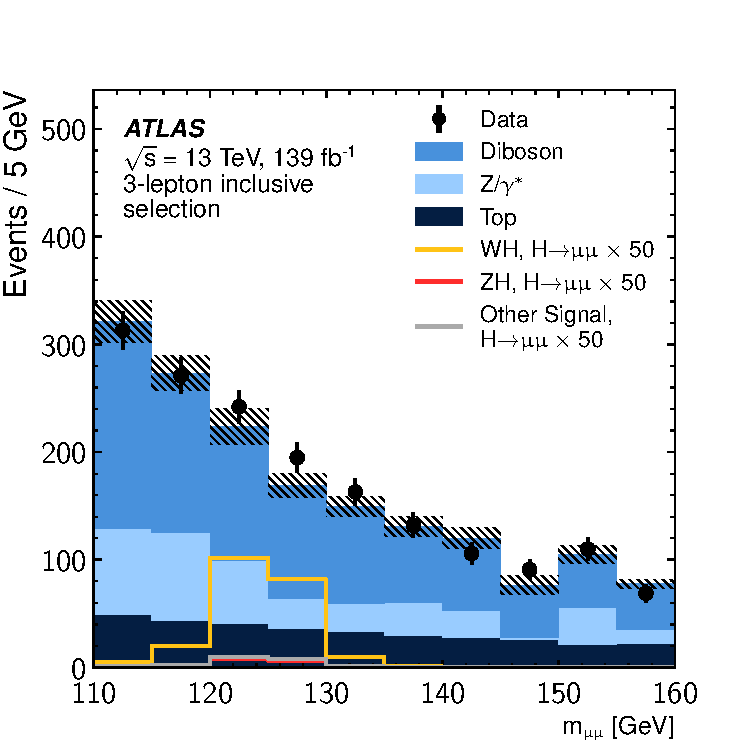
\includegraphics[width=0.5\textwidth]{figures/hmm/public/preCut/histo-3lep-muu.pdf}}}
\caption{Distributions of \muu in the 4-lepton (left) and 3-lepton (right) categories. The binning is adjusted based on the multiplicities of the categories. The signal distributions, shown in colored lines, are scaled by a factor of 50 for visibility.}
\label{fig:hmmPrecutMassHists}
\end{figure}

    
Other kinematic distributions ($p_T$, $\eta$, $\phi$) for the selected leptons are illustrated in Figures \ref{fig:hmmKineWhMuons} to \ref{fig:hmmKineZhLeps}.
The muon candidates for the Higgs are called $\mu^1$ and $\mu^2$ in descending order of $p_T$. 
Likewise, for the 4-lepton category, the selected leptons for the Z candidate are named $\ell^1$ and $\ell^2$ again in descending order of $p_T$.



\clearpage
\begin{figure}[htpb]
  \centering
  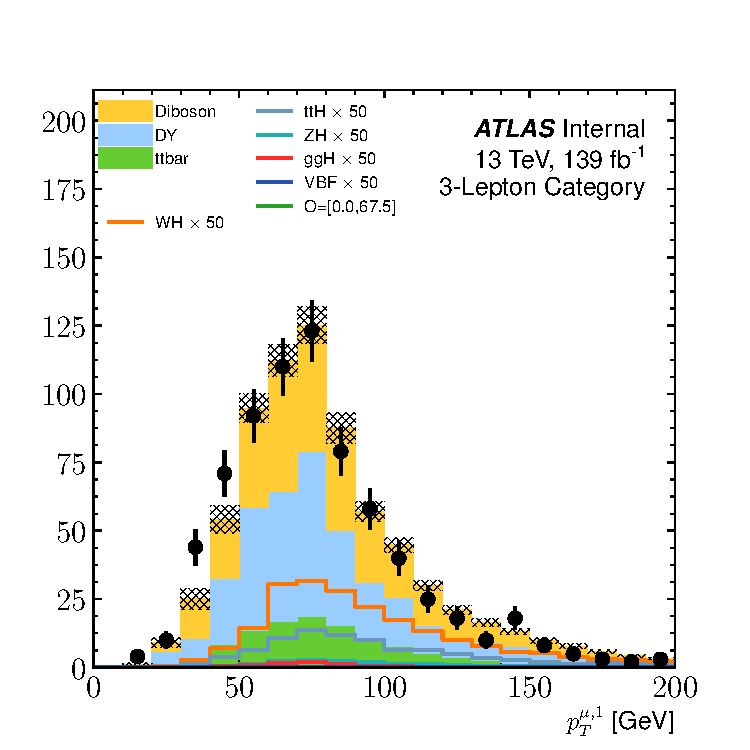
\includegraphics[width=0.4\textwidth]{figures/hmm/kinematics/histo-3lep-u1_pt.pdf}
  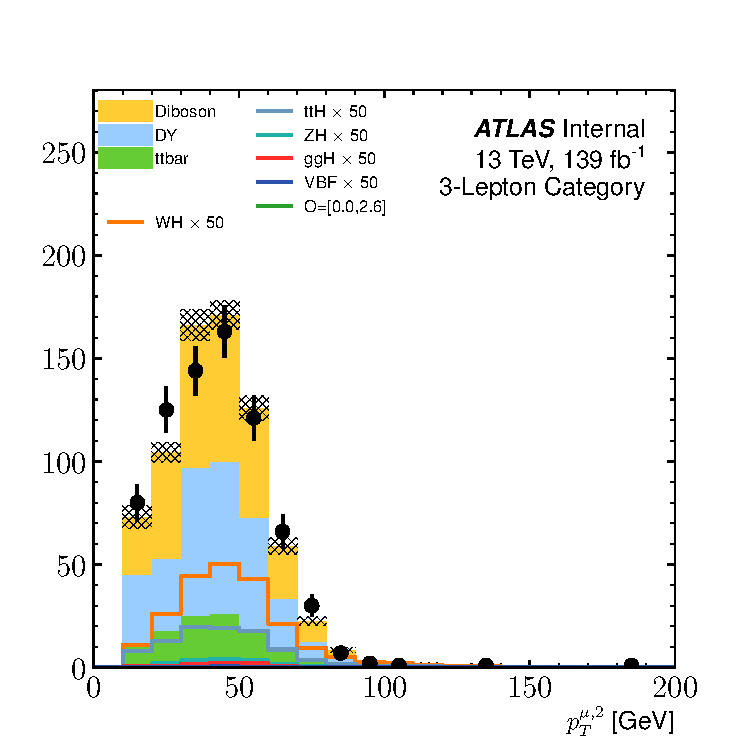
\includegraphics[width=0.4\textwidth]{figures/hmm/kinematics/histo-3lep-u2_pt.pdf}
  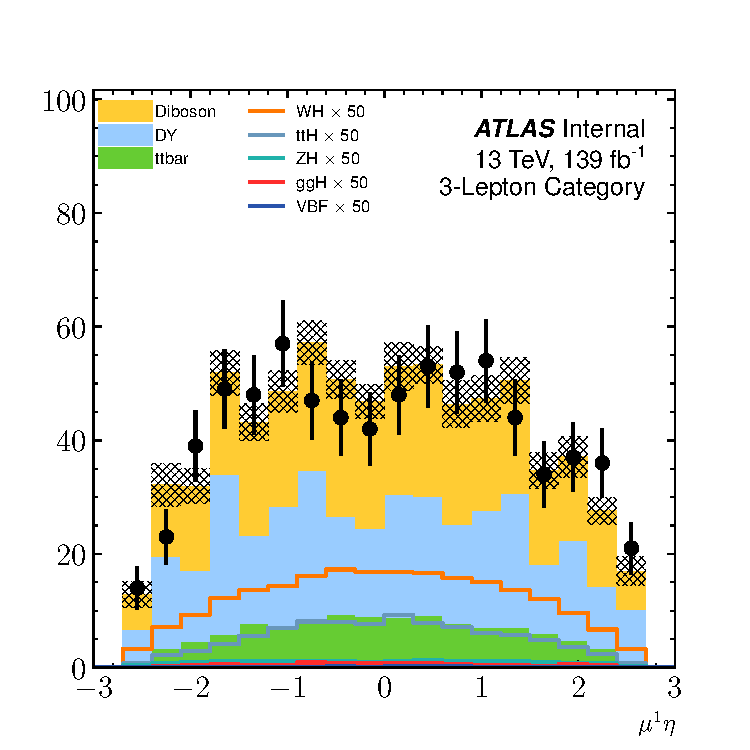
\includegraphics[width=0.4\textwidth]{figures/hmm/kinematics/histo-3lep-u1_eta.pdf}
  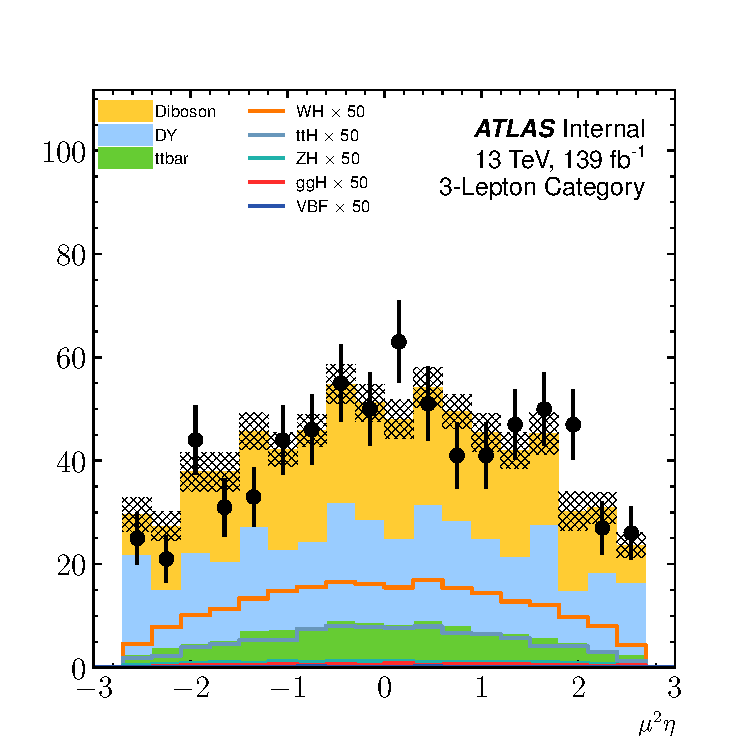
\includegraphics[width=0.4\textwidth]{figures/hmm/kinematics/histo-3lep-u2_eta.pdf}
  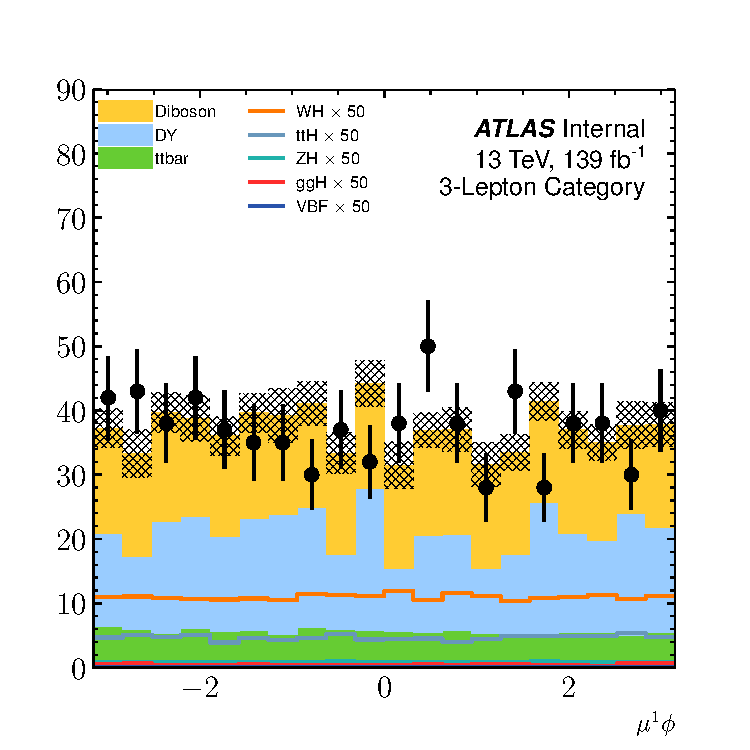
\includegraphics[width=0.4\textwidth]{figures/hmm/kinematics/histo-3lep-u1_phi.pdf}
  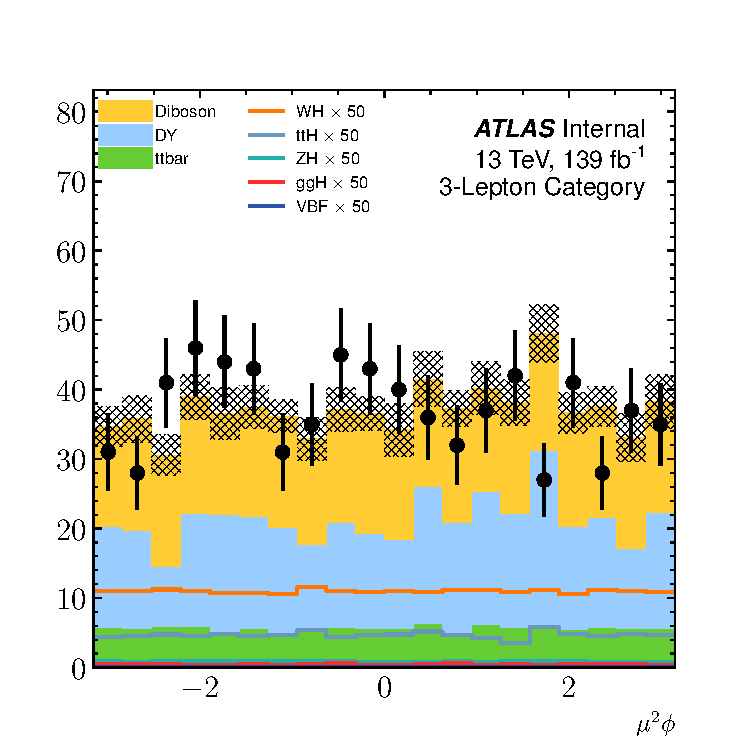
\includegraphics[width=0.4\textwidth]{figures/hmm/kinematics/histo-3lep-u2_phi.pdf}
  \caption{Kinematic plots showing $p_T$, $\eta$, and $\phi$ distributions for the H candidate muons from the 3-lepton selection.}
    \label{fig:hmmKineWhMuons}
\end{figure}

\clearpage
\begin{figure}[htpb]
  \centering
  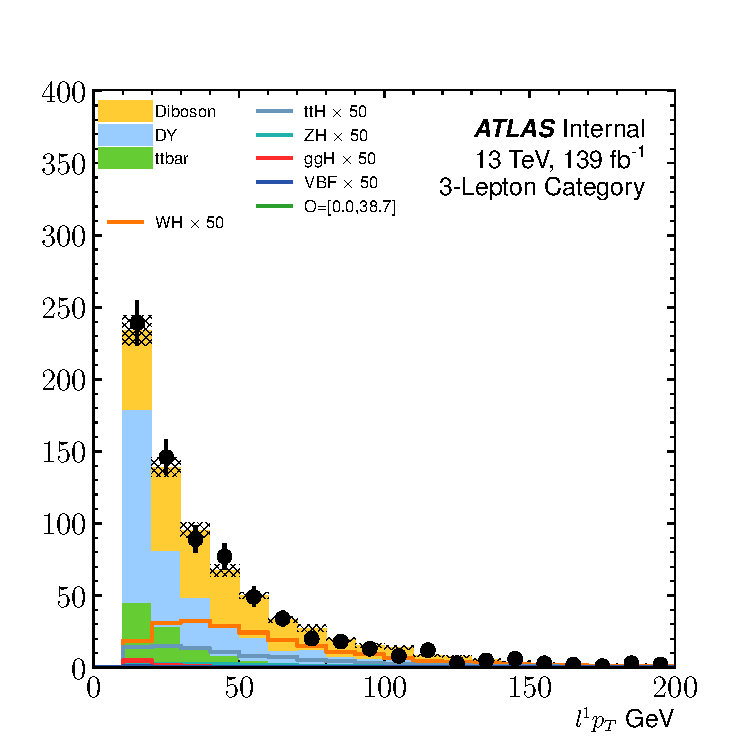
\includegraphics[width=0.4\textwidth]{figures/hmm/kinematics/histo-3lep-aux1_pt.pdf}\\
  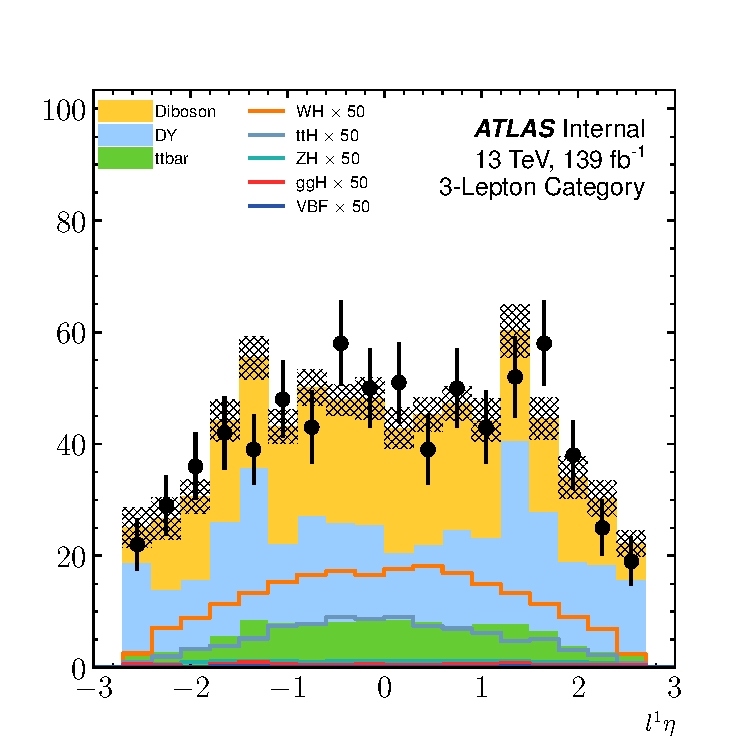
\includegraphics[width=0.4\textwidth]{figures/hmm/kinematics/histo-3lep-aux1_eta.pdf}\\
  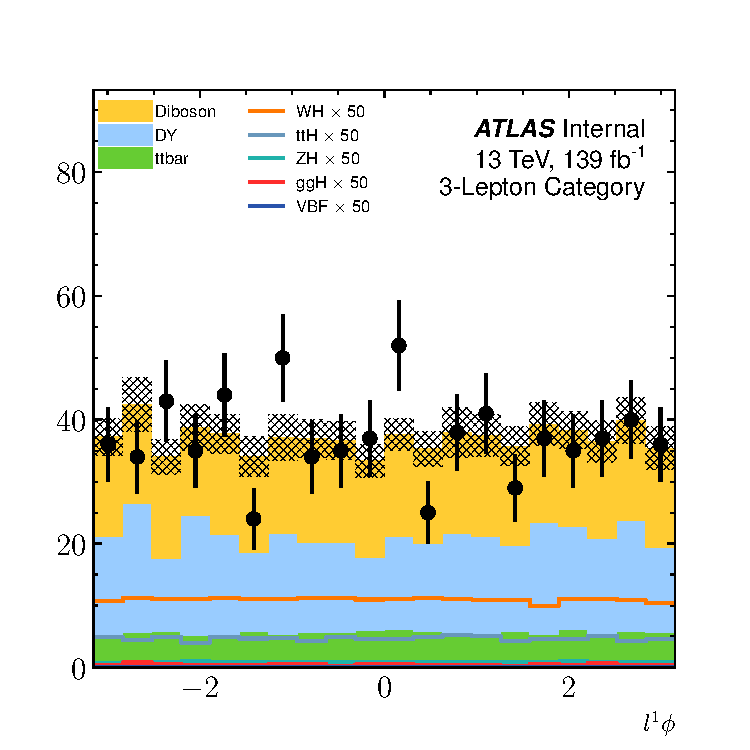
\includegraphics[width=0.4\textwidth]{figures/hmm/kinematics/histo-3lep-aux1_phi.pdf}\\
  \caption{Kinematic plots showing $p_T$, $\eta$, and $\phi$ distributions for the additional lepton/W candidate for the 3-lepton selection.}
    \label{fig:hmmKineWhLeps}
\end{figure}

\clearpage
\begin{figure}[htpb]
  \centering
  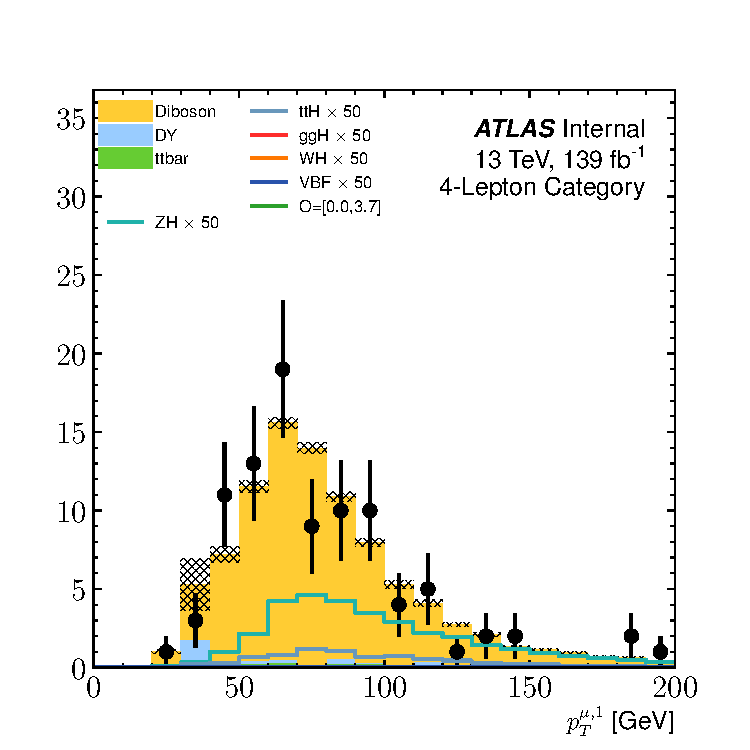
\includegraphics[width=0.4\textwidth]{figures/hmm/kinematics/histo-4lep-u1_pt.pdf}
  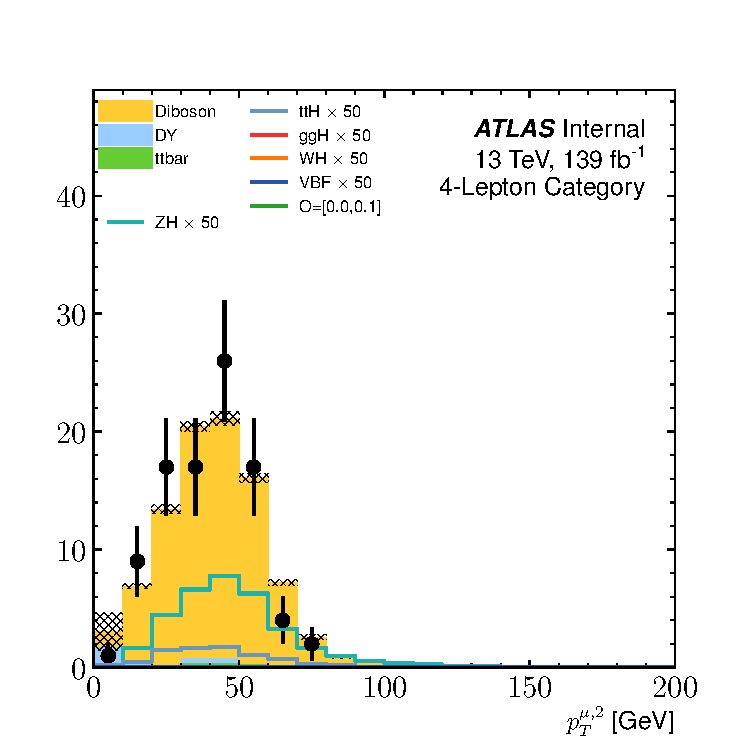
\includegraphics[width=0.4\textwidth]{figures/hmm/kinematics/histo-4lep-u2_pt.pdf}
  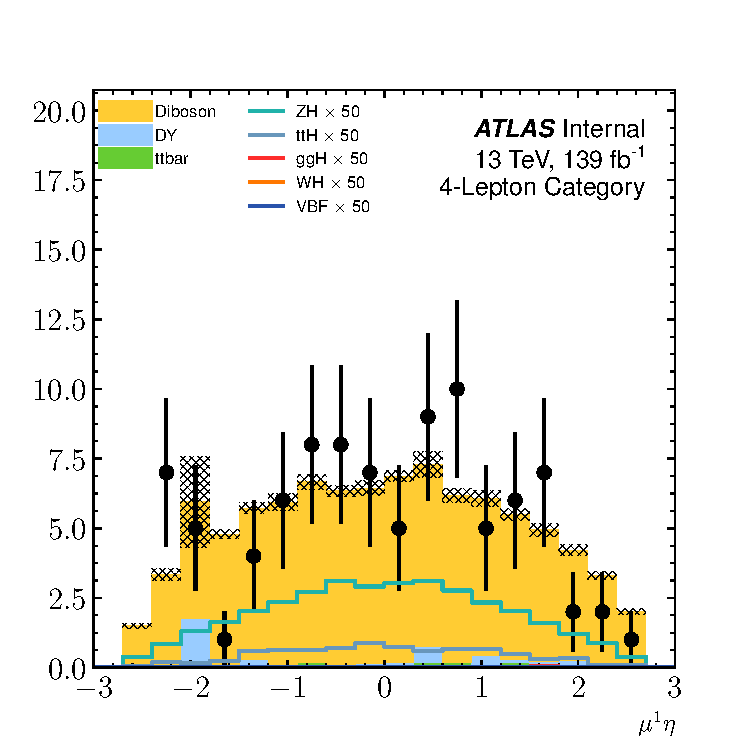
\includegraphics[width=0.4\textwidth]{figures/hmm/kinematics/histo-4lep-u1_eta.pdf}
  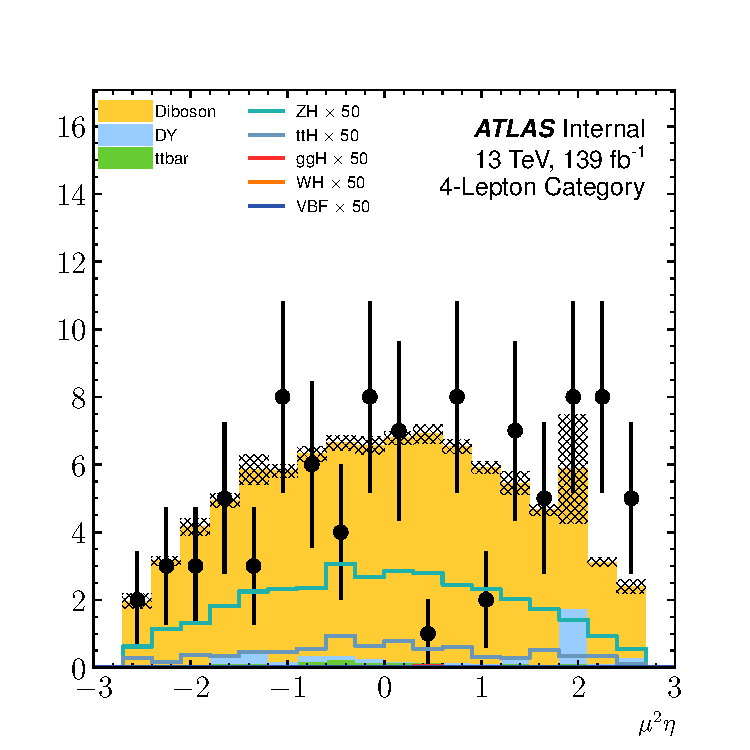
\includegraphics[width=0.4\textwidth]{figures/hmm/kinematics/histo-4lep-u2_eta.pdf}
  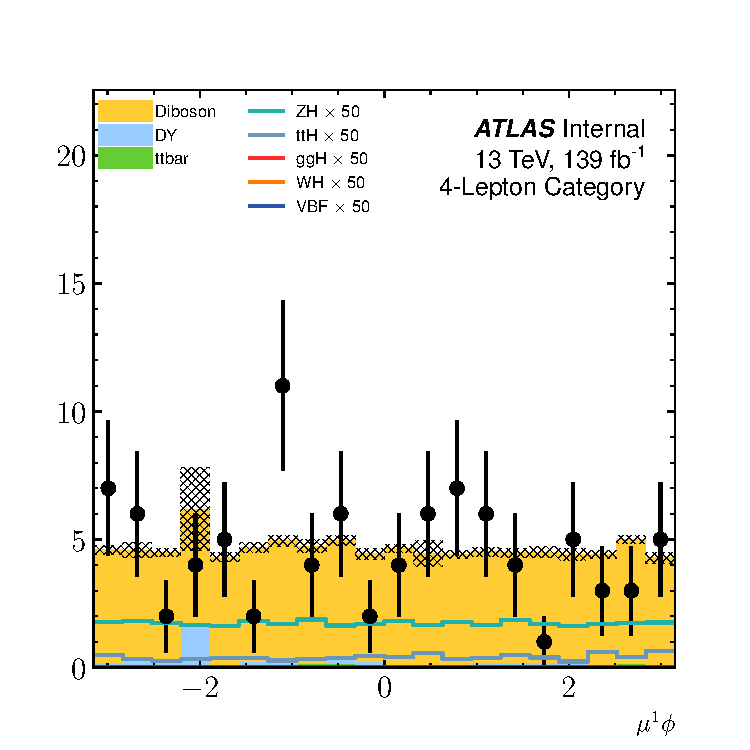
\includegraphics[width=0.4\textwidth]{figures/hmm/kinematics/histo-4lep-u1_phi.pdf}
  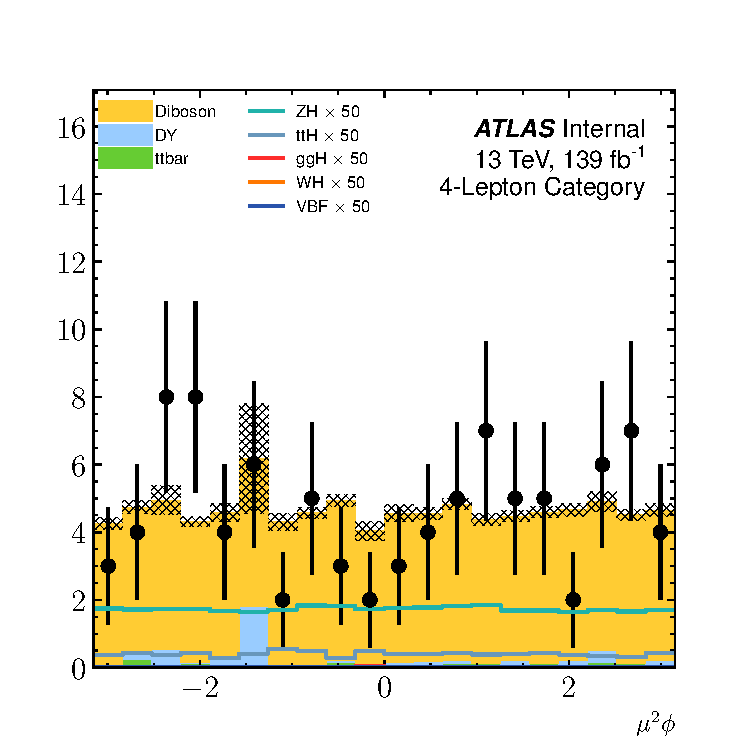
\includegraphics[width=0.4\textwidth]{figures/hmm/kinematics/histo-4lep-u2_phi.pdf}
  \caption{Kinematic plots showing $p_T$, $\eta$, and $\phi$ distributions for the H candidate muons from the 4-lepton selection.}
    \label{fig:hmmKineZhMuons}
\end{figure}

\clearpage
\begin{figure}[htpb]
  \centering
  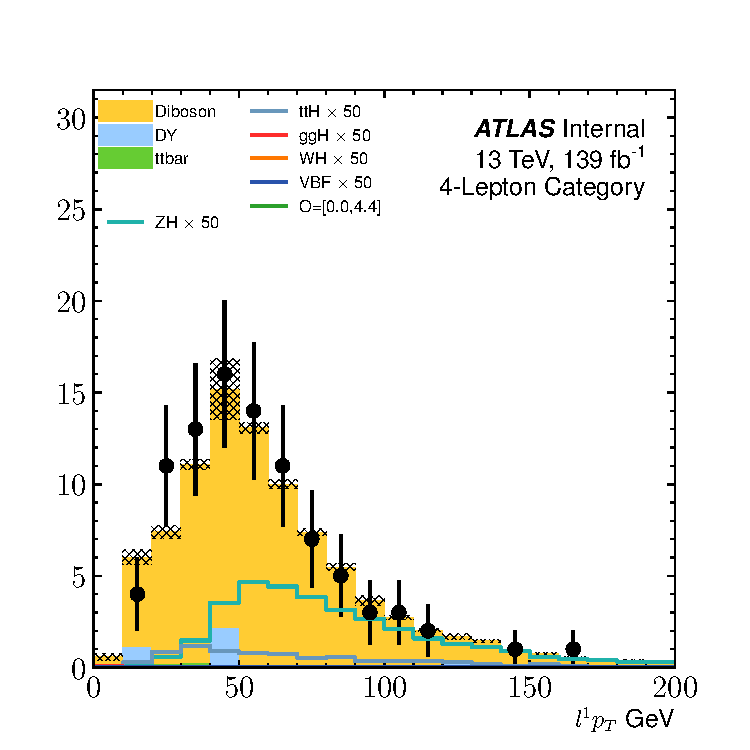
\includegraphics[width=0.4\textwidth]{figures/hmm/kinematics/histo-4lep-aux1_pt.pdf}
  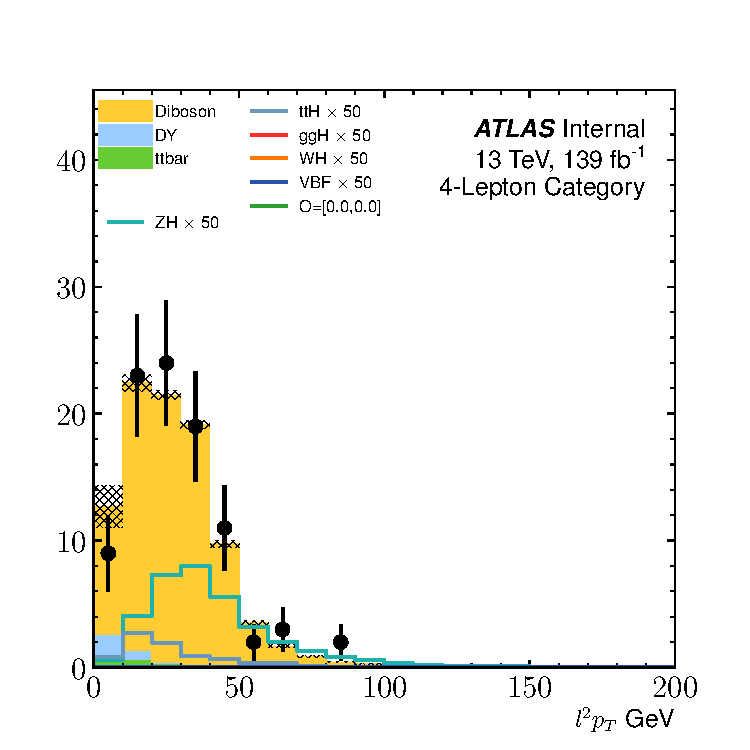
\includegraphics[width=0.4\textwidth]{figures/hmm/kinematics/histo-4lep-aux2_pt.pdf}
  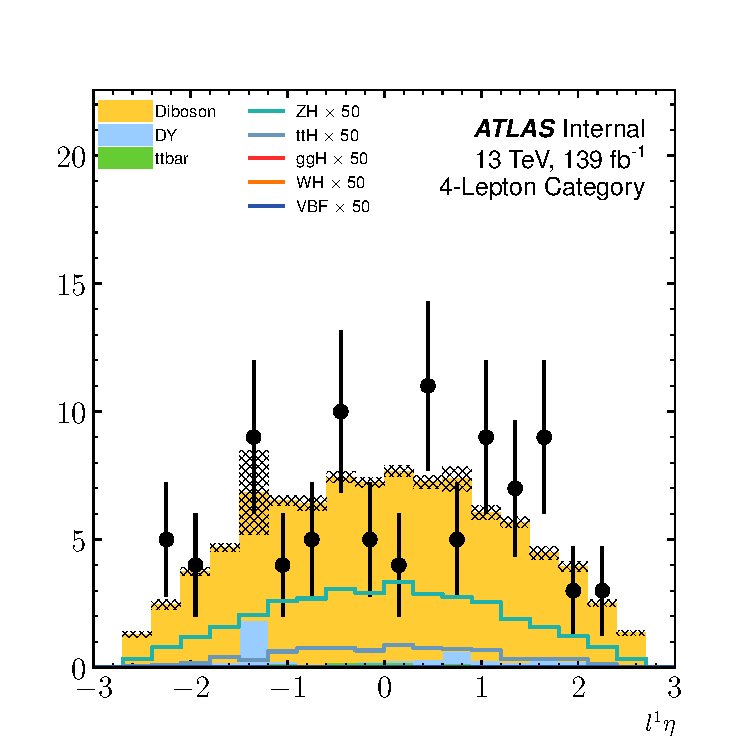
\includegraphics[width=0.4\textwidth]{figures/hmm/kinematics/histo-4lep-aux1_eta.pdf}
  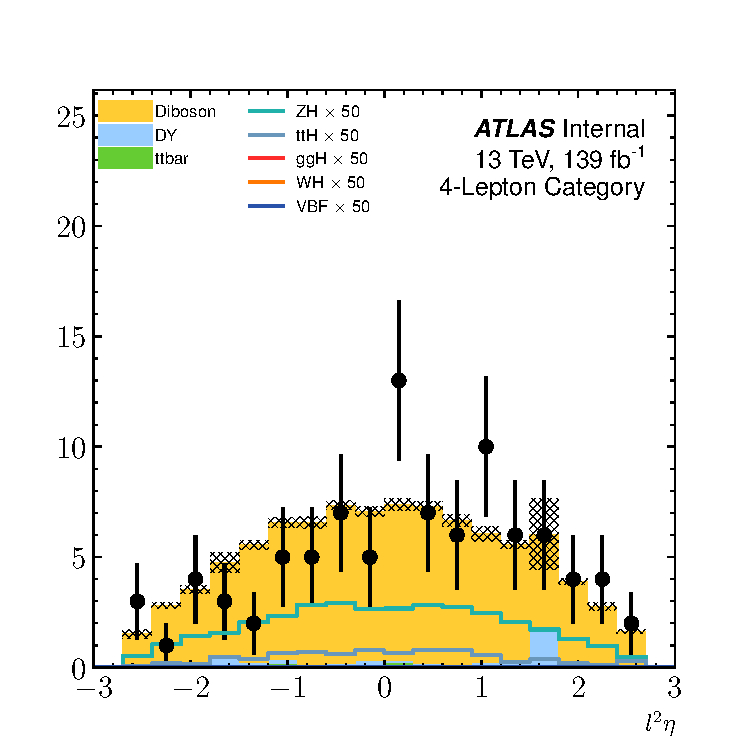
\includegraphics[width=0.4\textwidth]{figures/hmm/kinematics/histo-4lep-aux2_eta.pdf}
  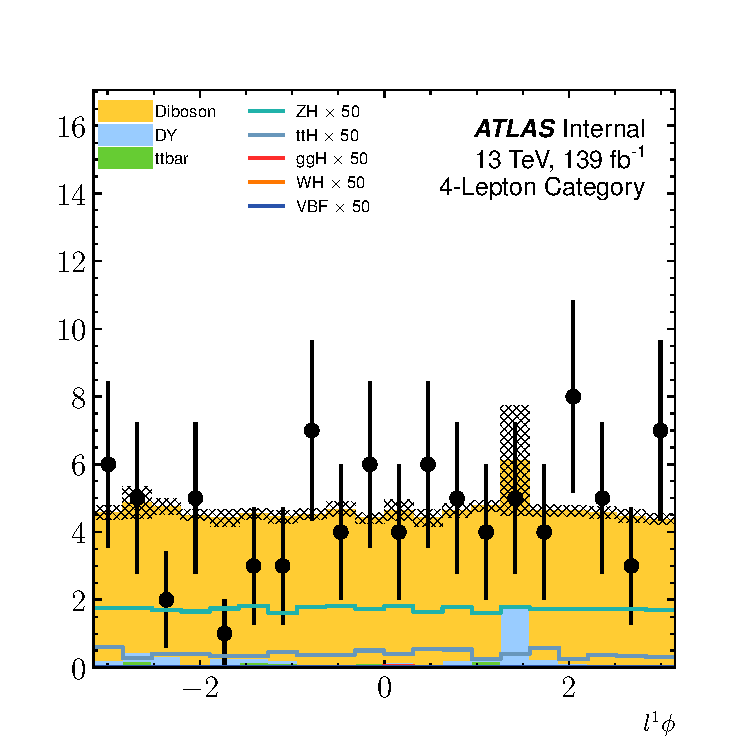
\includegraphics[width=0.4\textwidth]{figures/hmm/kinematics/histo-4lep-aux1_phi.pdf}
  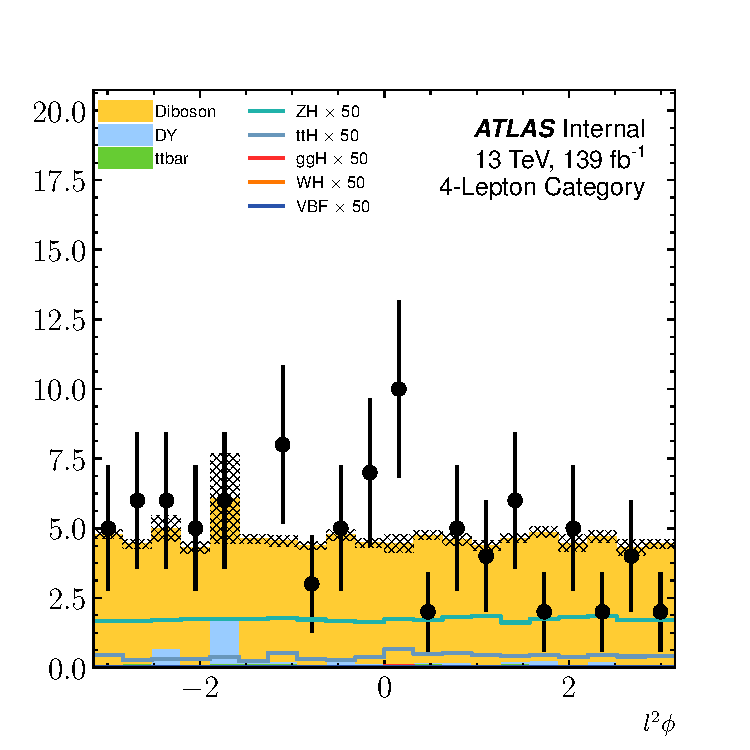
\includegraphics[width=0.4\textwidth]{figures/hmm/kinematics/histo-4lep-aux2_phi.pdf}
  \caption{Kinematic plots showing $p_T$, $\eta$, and $\phi$ distributions for the Z candidate leptons from the 4-lepton selection.}
    \label{fig:hmmKineZhLeps}
\end{figure}
\clearpage



\section{Multivariate Categorization}\label{sec:hmmBdt}

This section describes the separation of the ``pre-cut'' 3-lepton and 4-lepton categories into ``post-cut'' sub-categories in order to enhance the overall sensitivity.
Boosted decision trees (BDTs) are trained using the signal and background simulations in each of these categories.

\subsection{Configuration}
\label{sec:hmmBdtConfiguration}

% Training details
Different classifiers are used for both the 3-lepton and 4-lepton categories, but these share a common setup.
The classifier algorithm used is XGBoost.\cite{xgboost} 

A 5-fold splitting of the available signal and background sample is used.
 Three fifths of each sample define the \emph{training} sample used to fit the BDT.
 One fifth of the sample defines a \emph{validation} sample used to evaluate the performance of the BDT, control the potential for over training to the testing sample, and to select the cuts on the BDT output used for categorization.
 One fifth of the sample defines a \emph{testing} sample which remains blinded until the choices related to the VH channels have been fixed.
 The output of the BDT on the testing sample represent the final result of the BDT and it is essential to refrain from making choices related to the BDT performance on the testing set.
 For example, selecting an optimal cut using the BDT testing set, and then using the same testing set to estimate signal strength, will result in an expected signal amplitude that is larger than that from an unexposed sample 
(e.g. data).
 Making such choices using the \emph{validation} sample avoids this particular complication.

Cross validation is was introduced in order to maximise the benefit from the limited statistics available in simulated events. A cyclic permutation of the 5-fold splitting is used, such that a separate BDT is trained for each fifth of the total sample.

% Samples
Each BDT is trained using the simulated background, with all background components included in the training sample.
The signal for the 4-lepton BDTs are the qqZH samples, while the signal for the 3-lepton BDTs are the W$^\pm$H samples. The per-event weights arising from scale factors and reweighing, along with the event corresponding to the campaign luminosity, cross section, etc are provided to the BDT. Negatively weighted events are removed, and the signal and background weights are both normalized.

% Sample statistics
The available events for training are shown in table \ref{tab:hmmSampleStatistics}.

\begin{table}[htbp]
 \begin{center}
\begin{tabular}{l r r r}\toprule
Sample               & Total Events & Training Events \\
4-lepton signal      & 20700        & 12508    \\
4-lepton background  & 88314        & 53081    \\
3-lepton signal      & 134936       & 80962    \\
3-lepton background  & 185286       & 111107   \\
\bottomrule\end{tabular} 
 \end{center}
 \caption{Numbers of MC events available for training, both in the full sample, and the 3/5 training sample statistics.}
\label{tab:hmmSampleStatistics}
\end{table}

% Training variables
The set of variables provided as input for the BDT was chosen from a larger set of candidate variables.
This set was reduced in order of ascending feature importance (measured by the number of times the variable is used for a decision weighted by the events categorized by the node) until the BDT performance suffers (measured by the AUC).
Different variables are present for the 4-lepton and 3-lepton categories.
The variables for each are listed in Tables \ref{tab:hmm3lepVars} and \ref{tab:hmm4lepVars}.

\begin{table}[htp]
\begin{center}
\begin{tabular}{l l l l}
\toprule
Variable & Definition \\
\midrule
 $\Delta_\phi(E_T^\text{miss},H)$ & $\phi$ between $E_T^\text{miss}$ and the H candidate \\
 $p_T^{l1}$ & W candidate lepton $p_T$ \\
 $m_T(E_T^\text{miss},l1)$ & transverse mass of the W candidate lepton and $E_T^\text{miss}$  \\
 $\Delta_\phi(l1,H)$ & $\Delta$ $\phi$ between H candidate and W candidate lepton \\
 $\Delta_\eta(l1,H)$ & $\Delta$ $\eta$ between H candidate and W candidate lepton \\
 $E_T^\text{miss}$ & missing transverse momentum \\
 $p_T^{j1}$ & $p_T$ of leading jet (if present) \\
 $N_\text{jets}$ & Number of jets \\
\bottomrule
\end{tabular}
\caption{3-lepton variables.}
\label{tab:hmm3lepVars}
\end{center}
\end{table}

\begin{table}[htp]
\begin{center}
\begin{tabular}{l l l l}
\toprule
Variable & Definition \\
\midrule
 $p_T^{j1}$ & $p_T$ of leading jet (if present) \\
 $p_T^{j2}$ & $p_T$ of subleading jet (if present) \\
 $N_\text{jets}$ & Number of jets \\
 $\Delta_\phi(l1,l2)$ & $\Delta$ $\phi$ between the leptons paired for the Z candidate \\
 $\Delta_\phi(Z,H)$ & $\Delta$ $\phi$ between H candidate and Z candidate \\
 $\Delta_\eta(Z,H)$ & $\Delta$ $\eta$ between H candidate and Z candidate \\
 $m_Z$ & Z candidate mass \\
\bottomrule
\end{tabular}
\caption{4-lepton variable.}
\label{tab:hmm4lepVars}
\end{center}
\end{table}

\afterpage{
\begin{figure}[h!]
\captionsetup[subfigure]{position=b}
\centering
\subfloat[][]{{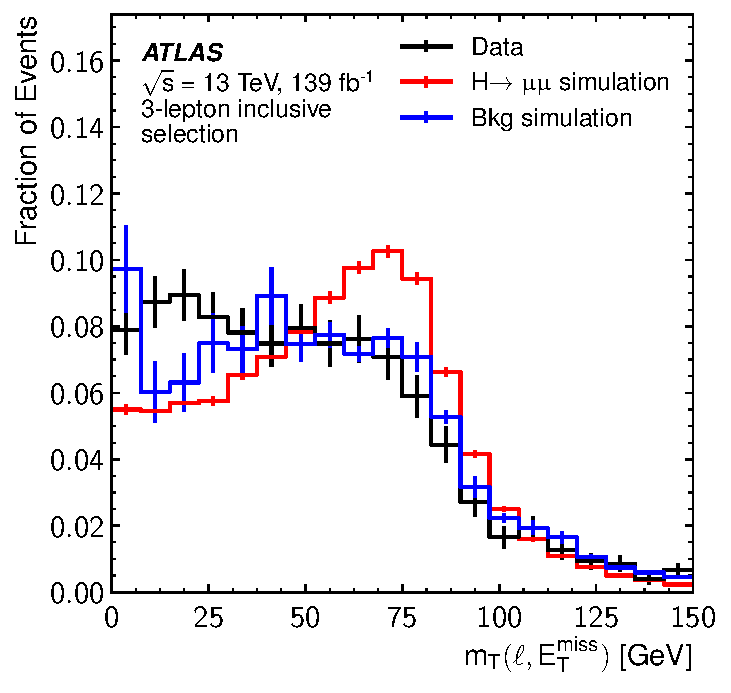
\includegraphics[width=0.35\textwidth]{/home/prime/thesis/draft-text-030820/figures/hmm/public/kine/kine-3lep-aux1_met_mt.pdf}}}
\subfloat[][]{{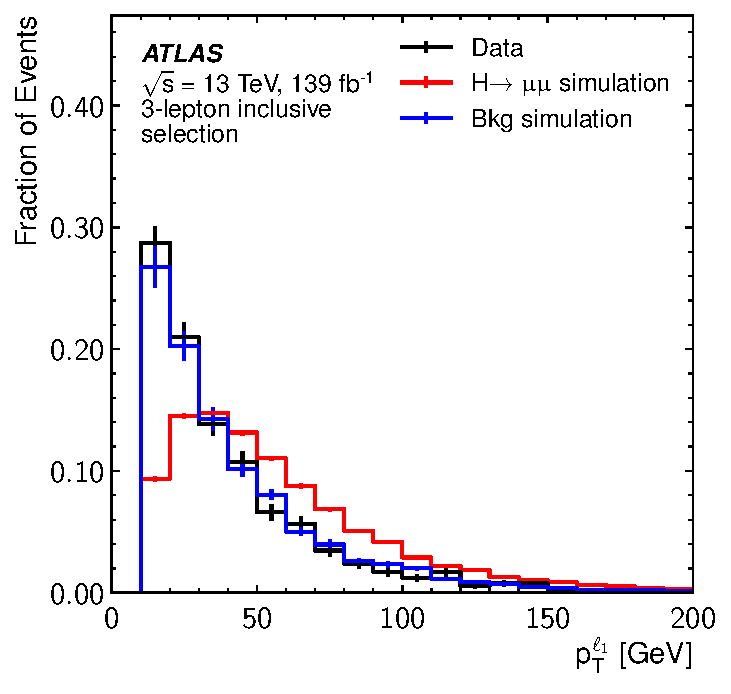
\includegraphics[width=0.35\textwidth]{/home/prime/thesis/draft-text-030820/figures/hmm/public/kine/kine-3lep-aux1_pt.pdf}}}
\subfloat[][]{{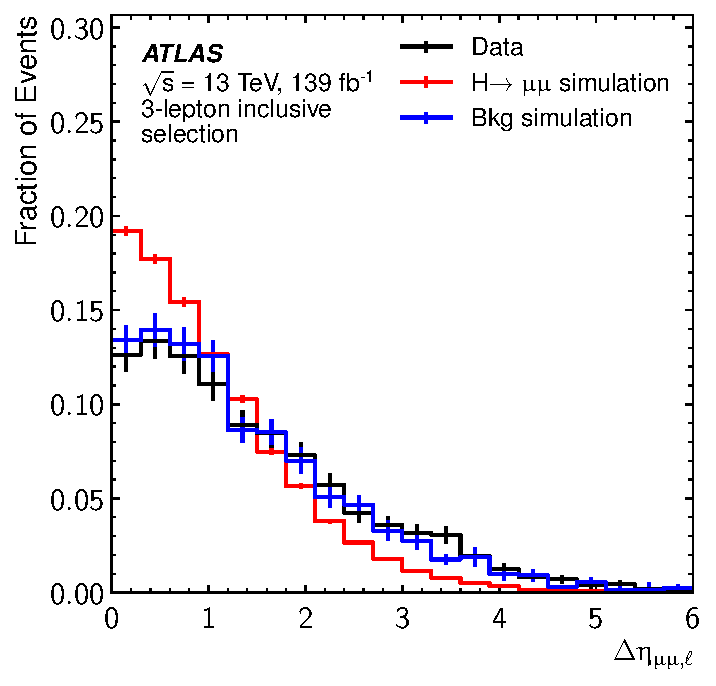
\includegraphics[width=0.35\textwidth]{/home/prime/thesis/draft-text-030820/figures/hmm/public/kine/kine-3lep-aux1_uu_delta_eta.pdf}}} \\
\subfloat[][]{{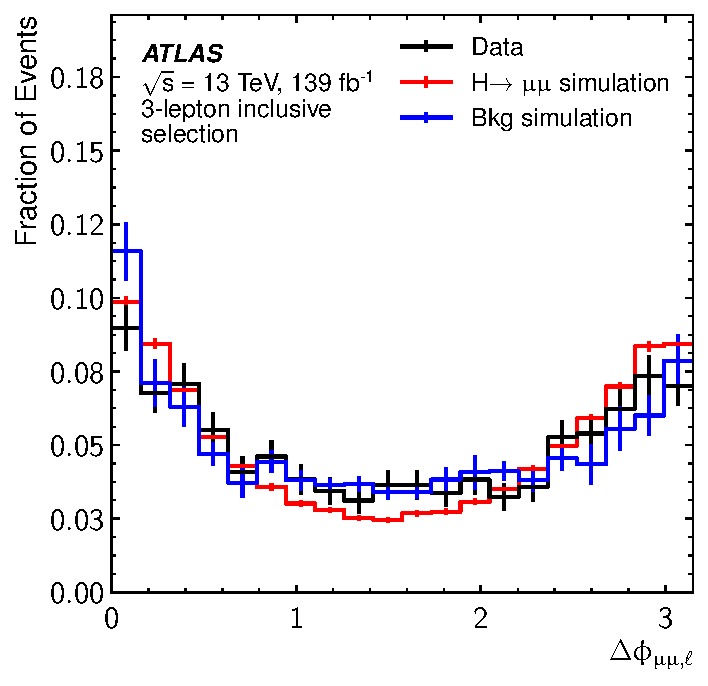
\includegraphics[width=0.35\textwidth]{/home/prime/thesis/draft-text-030820/figures/hmm/public/kine/kine-3lep-aux1_uu_delta_phi.pdf}}}
\subfloat[][]{{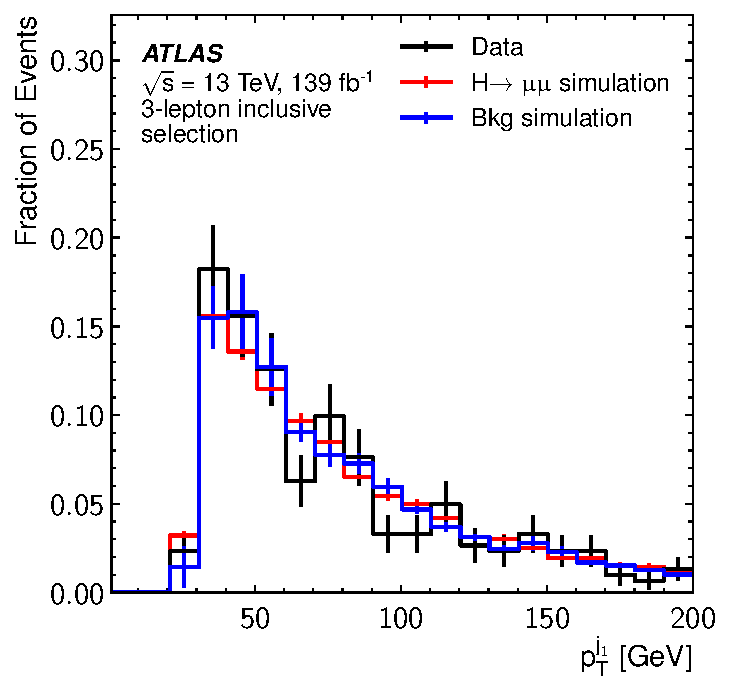
\includegraphics[width=0.35\textwidth]{/home/prime/thesis/draft-text-030820/figures/hmm/public/kine/kine-3lep-j1_pt.pdf}}}
\subfloat[][]{{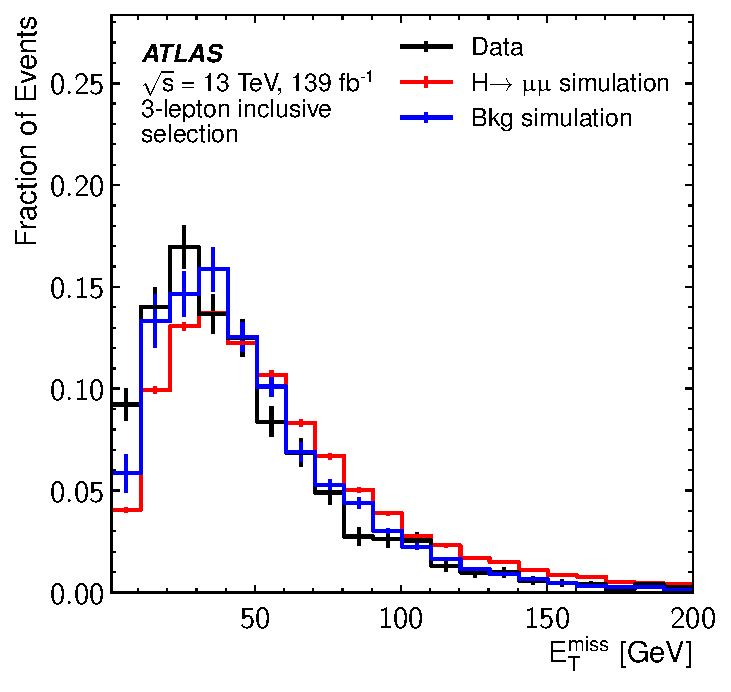
\includegraphics[width=0.35\textwidth]{/home/prime/thesis/draft-text-030820/figures/hmm/public/kine/kine-3lep-met_pt.pdf}}} \\
\subfloat[][]{{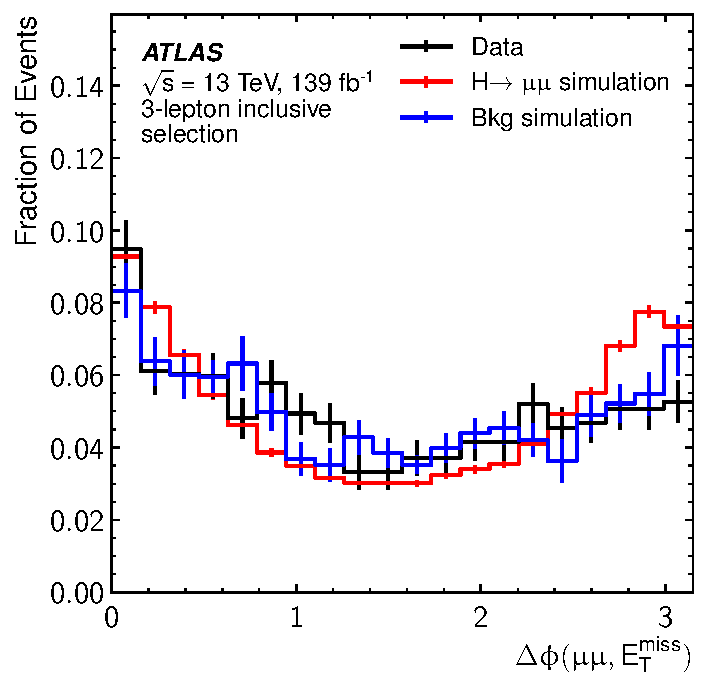
\includegraphics[width=0.35\textwidth]{/home/prime/thesis/draft-text-030820/figures/hmm/public/kine/kine-3lep-met_uu_delta_phi.pdf}}}
\subfloat[][]{{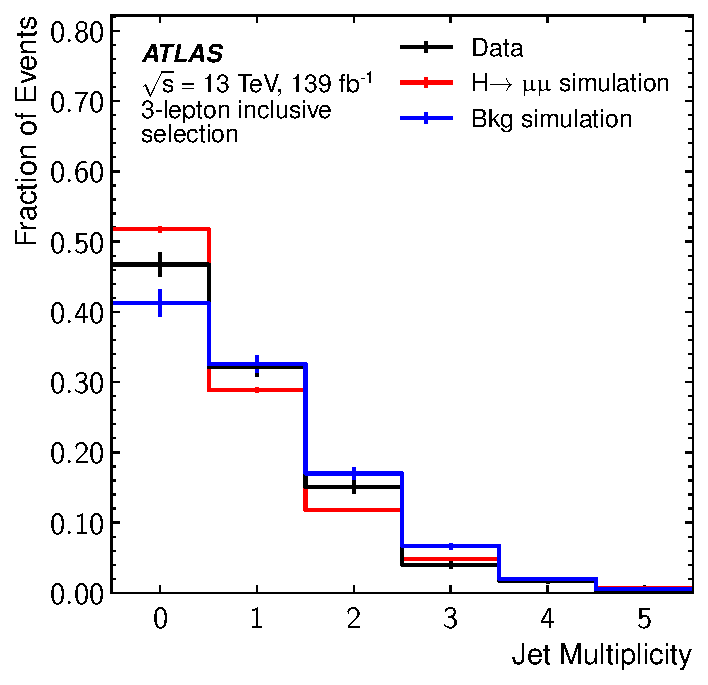
\includegraphics[width=0.35\textwidth]{/home/prime/thesis/draft-text-030820/figures/hmm/public/kine/kine-3lep-nJets.pdf}}}
\caption{Training variables provided as input for the for the 3-lepton classifier. The signal distribution shown in red is comprised of specifically the simulated WH signal dataset, while the background distribution contains all background shown in blue production modes. Data distributions are included in black. Each distribution is normalized, and the error bars on each histogram are statistical only. }
\label{fig:hmm3lepVars}
\end{figure}
\clearpage
}

\afterpage{
\begin{figure}[h!]
\captionsetup[subfigure]{position=b}
\centering
\subfloat[][]{{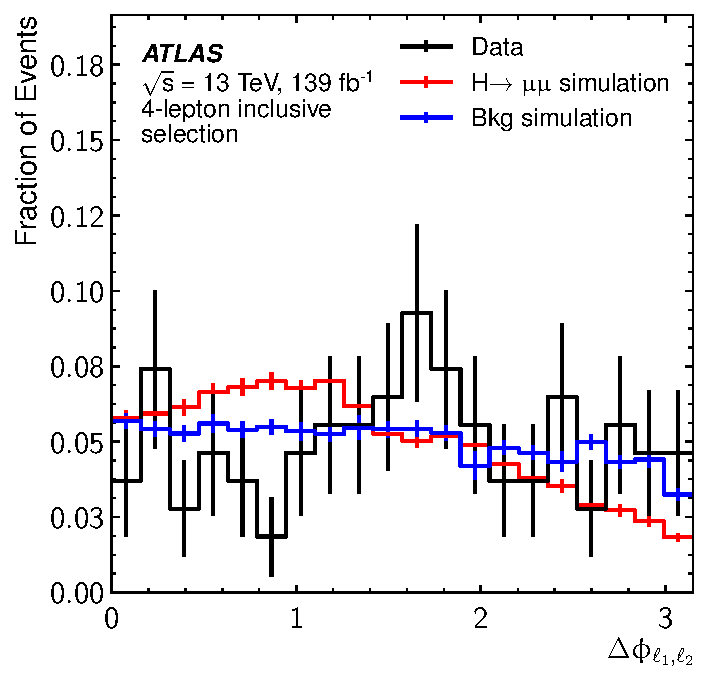
\includegraphics[width=0.35\textwidth]{/home/prime/thesis/draft-text-030820/figures/hmm/public/kine/kine-4lep-auxDilep_delta_phi.pdf}}}
\subfloat[][]{{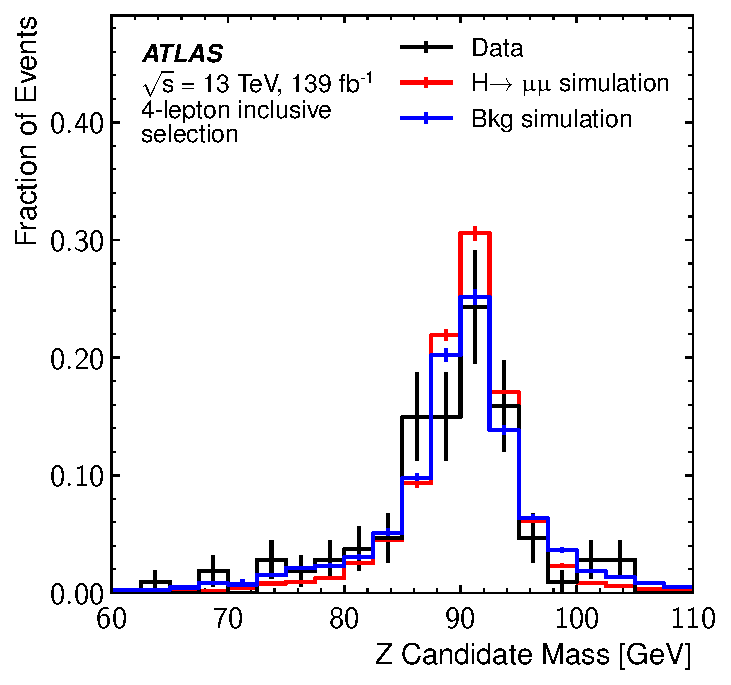
\includegraphics[width=0.35\textwidth]{/home/prime/thesis/draft-text-030820/figures/hmm/public/kine/kine-4lep-auxDilep_mass.pdf}}}
\subfloat[][]{{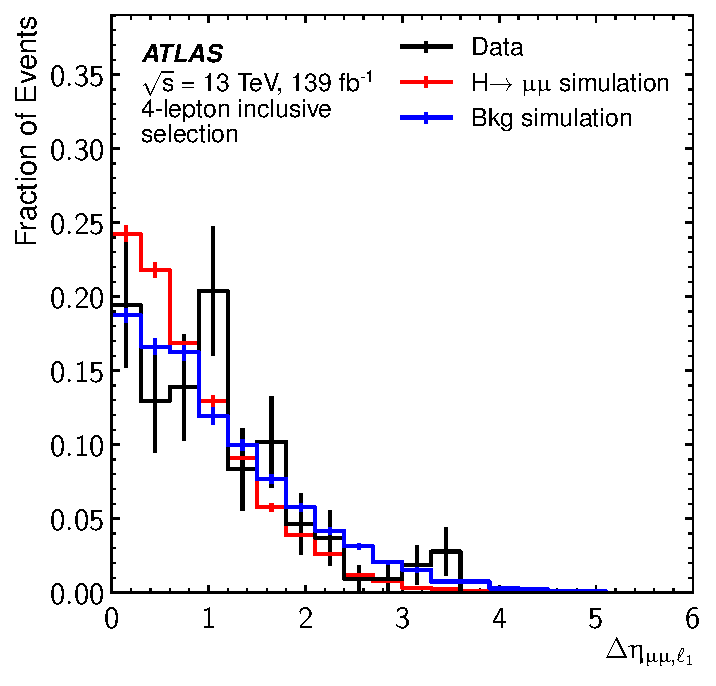
\includegraphics[width=0.35\textwidth]{/home/prime/thesis/draft-text-030820/figures/hmm/public/kine/kine-4lep-aux_uu_delta_eta.pdf}}} \\
\subfloat[][]{{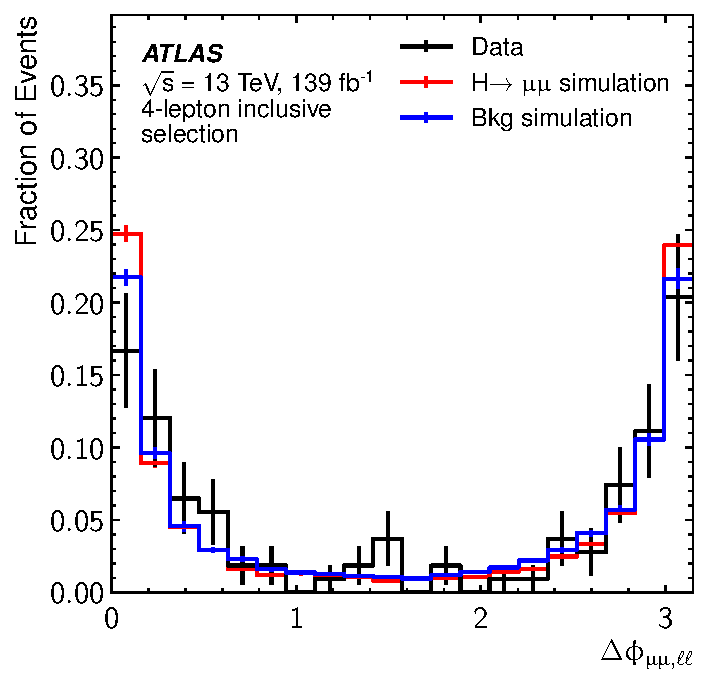
\includegraphics[width=0.35\textwidth]{/home/prime/thesis/draft-text-030820/figures/hmm/public/kine/kine-4lep-aux_uu_delta_phi.pdf}}}
\subfloat[][]{{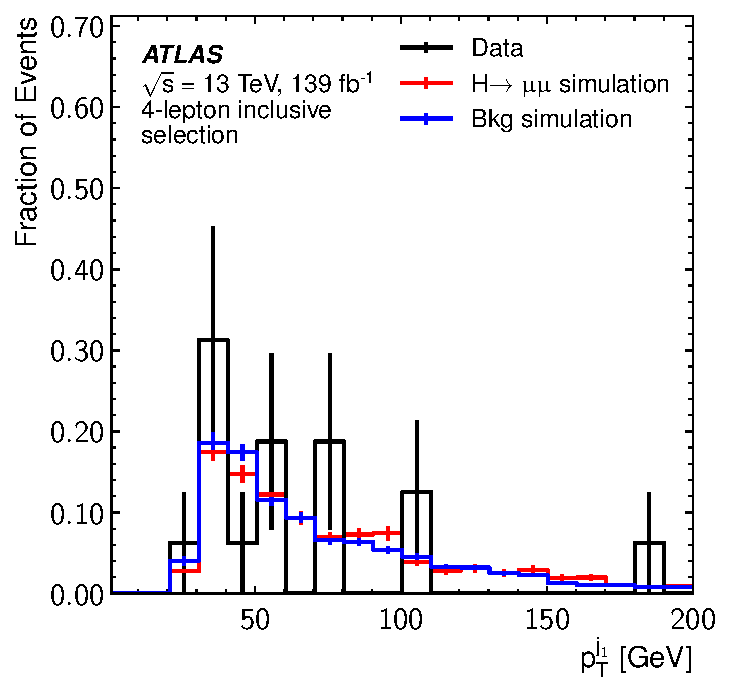
\includegraphics[width=0.35\textwidth]{/home/prime/thesis/draft-text-030820/figures/hmm/public/kine/kine-4lep-j1_pt.pdf}}}
\subfloat[][]{{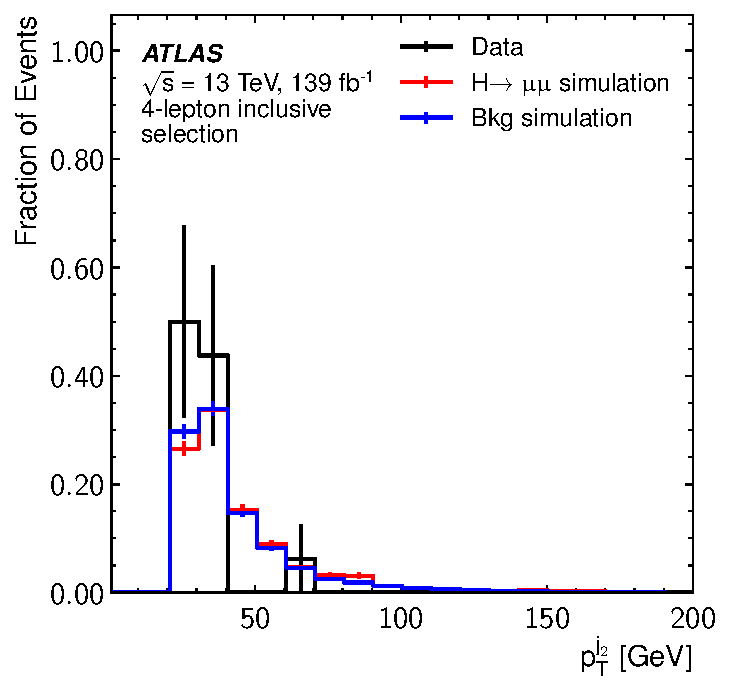
\includegraphics[width=0.35\textwidth]{/home/prime/thesis/draft-text-030820/figures/hmm/public/kine/kine-4lep-j2_pt.pdf}}} \\
\subfloat[][]{{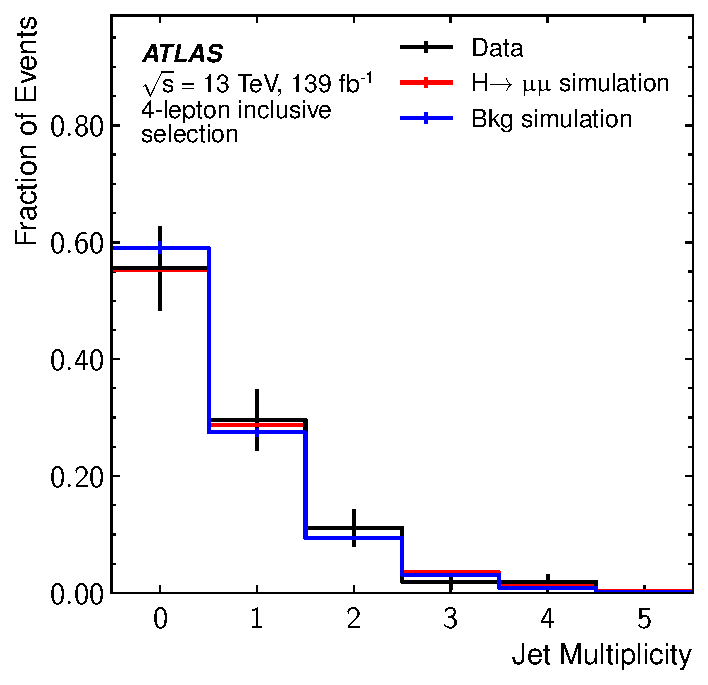
\includegraphics[width=0.35\textwidth]{/home/prime/thesis/draft-text-030820/figures/hmm/public/kine/kine-4lep-nJets.pdf}}}
\caption{Training variables provided as input for the for the 4-lepton classifier. The signal distribution shown in red is comprised of specifically the simulated WH signal dataset, while the background distribution contains all background shown in blue production modes. Data distributions are included in black. Each distribution is normalized, and the error bars on each histogram are statistical only. }
\label{fig:hmm4lepVars}
\end{figure}
\clearpage
}


%%%%%%%%%%%% Variable importance

\begin{figure}[htpb]
  \centering
  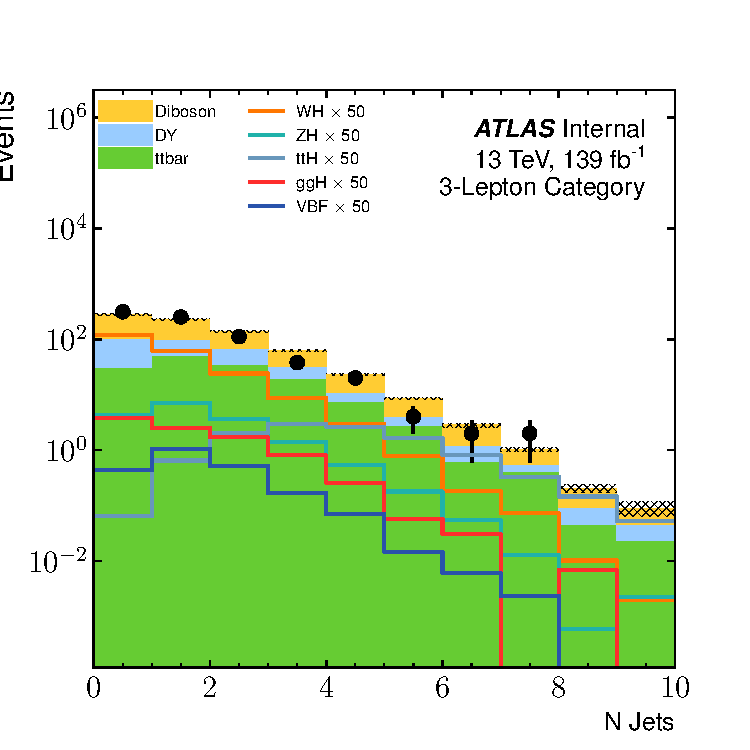
\includegraphics[height=0.48\textwidth]{figures/hmm/nJets/histo-3lep-nJets.pdf}
  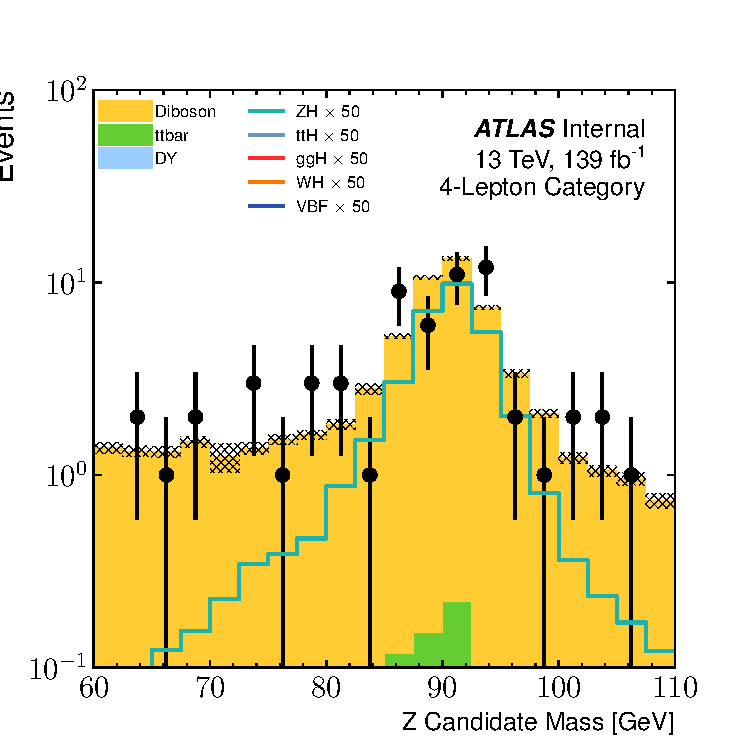
\includegraphics[height=0.48\textwidth]{figures/hmm/zCand/histo-4lep-auxDilep_mass.pdf}
  \caption{Left: N Jets distribution for 3-lepton channel, right: Z candidate mass for 4-lepton channel. These are the highest ranked in feature importance for their category's respective BDT's.}
    \label{fig:hmmImpVars}
\end{figure}

The importance of the variables used in the training are shown in the plots of figure \ref{fig:hmmVarImport}.
In the 4-lepton case, the most important variable is the mass of the Z candidate, which helps identify signal.
In the 3-lepton case the most important variable is the number of jets which helps to separate out Top backgrounds.
The distributions of these two variables are shown in figure \ref{fig:hmmImpVars}.
Detailed definition: \href{https://scikit-learn.org/stable/modules/feature_selection.html}{\underline{here}}.

\begin{figure}[htpb]
  \centering
  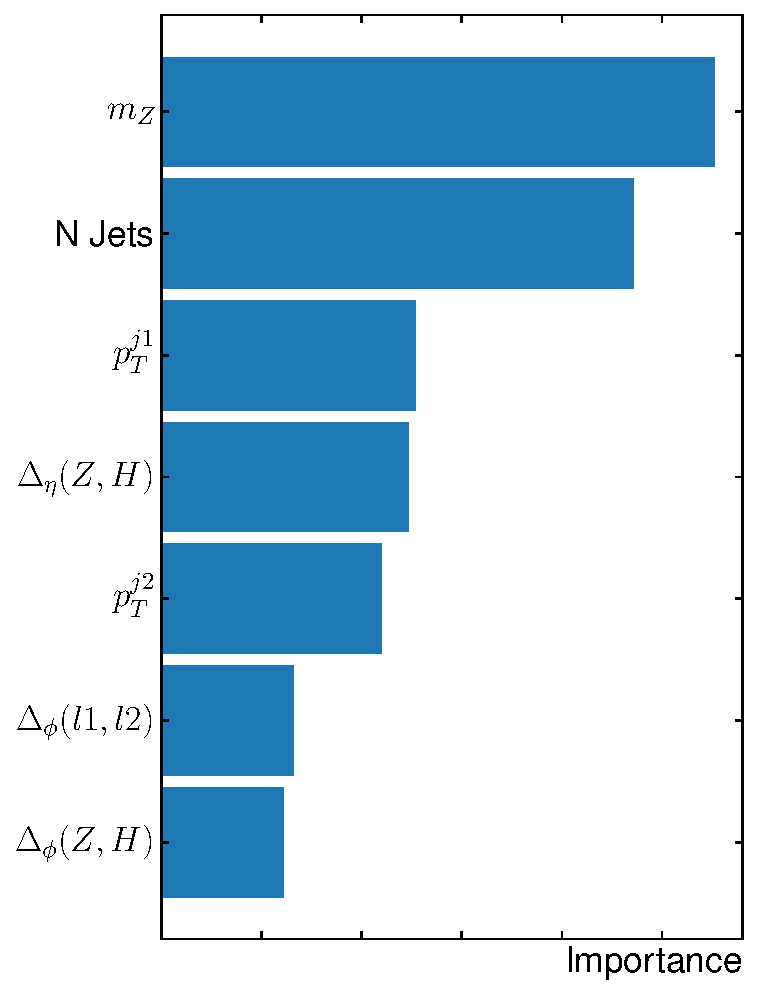
\includegraphics[height=7cm]{figures/hmm/bdtImportance/imp-4lep.pdf}
  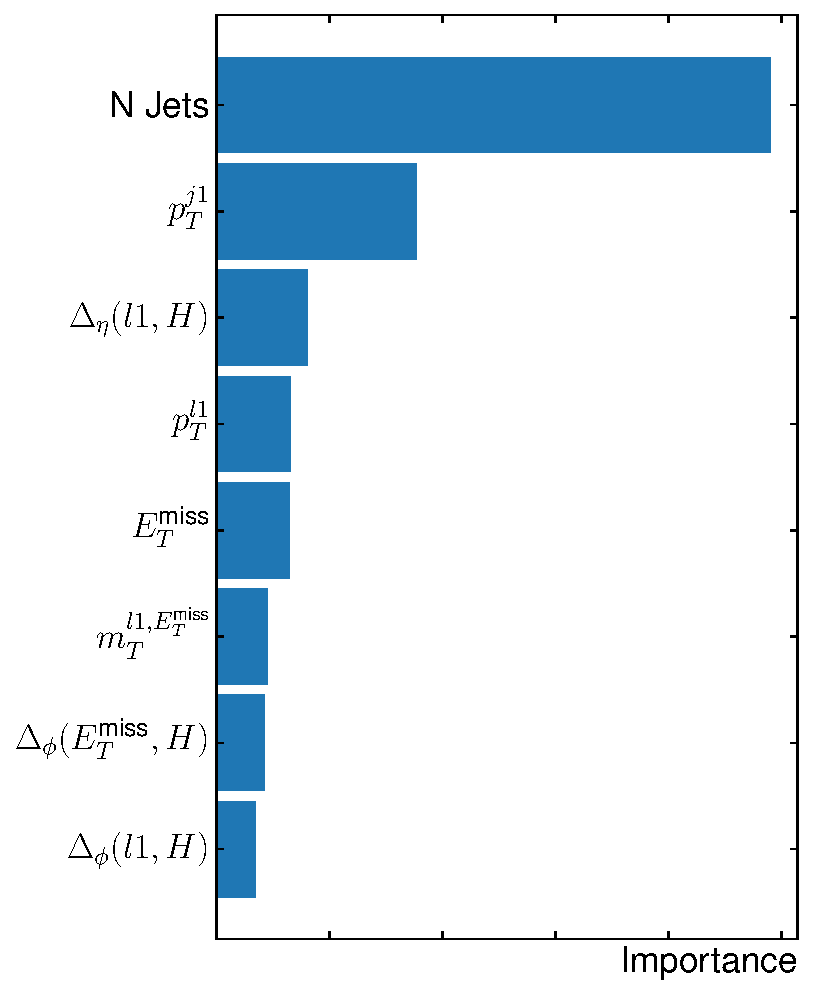
\includegraphics[height=7cm]{figures/hmm/bdtImportance/imp-3lep.pdf}
  \caption{The 4-lepton (left) and 3-lepton (right) variables shown with their respective feature importance, summed over each of the five BDT's trained for each cross validation permutation. $H$ stands for the Higgs candidate, $Z$ for the Z candidate, $l$ for the additional leptons in the event, and $j$ for the jets in the event. The number after the lepton or jet corresponds to the rank of it's $p_T$.}
    \label{fig:hmmVarImport}
\end{figure}

\clearpage

\subsection{Performance}
\label{sec:hmmBdtPerform}

The figure of merit for judging the BDT performance is the area under the receiver operating characteristic (ROC) curve (AUC). The ROC's for representative BDT's are shown for both 3- and 4-lepton categories in figure \ref{fig:hmmBdtRoc}. These show comparable performance for the BDT's of both categories, as well as the impact of the relatively limited statistics of the 4-lepton sample. The signal and background samples shown in the ROC plots correspond to the same samples used for the training, so only WH and ZH signals are shown.

\begin{figure}[htpb]
  \centering
  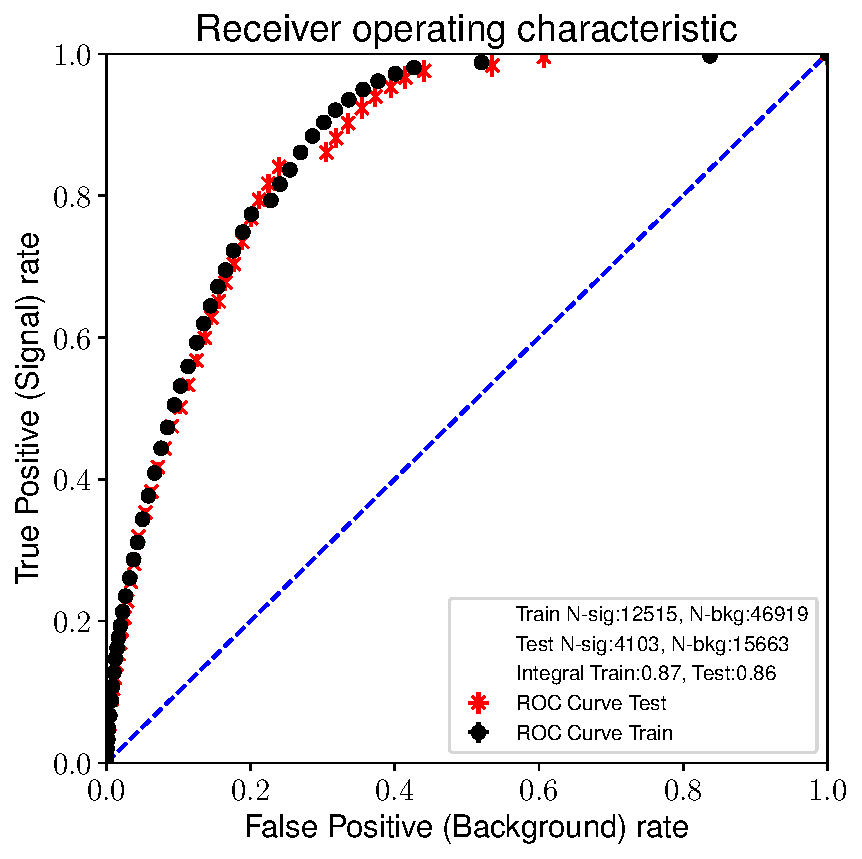
\includegraphics[width=0.48\textwidth]{figures/hmm/bdtHist/roc-4lep-ZH-AllBackground-0-depth2-nEst80tag-new-AllBackground.pdf}
  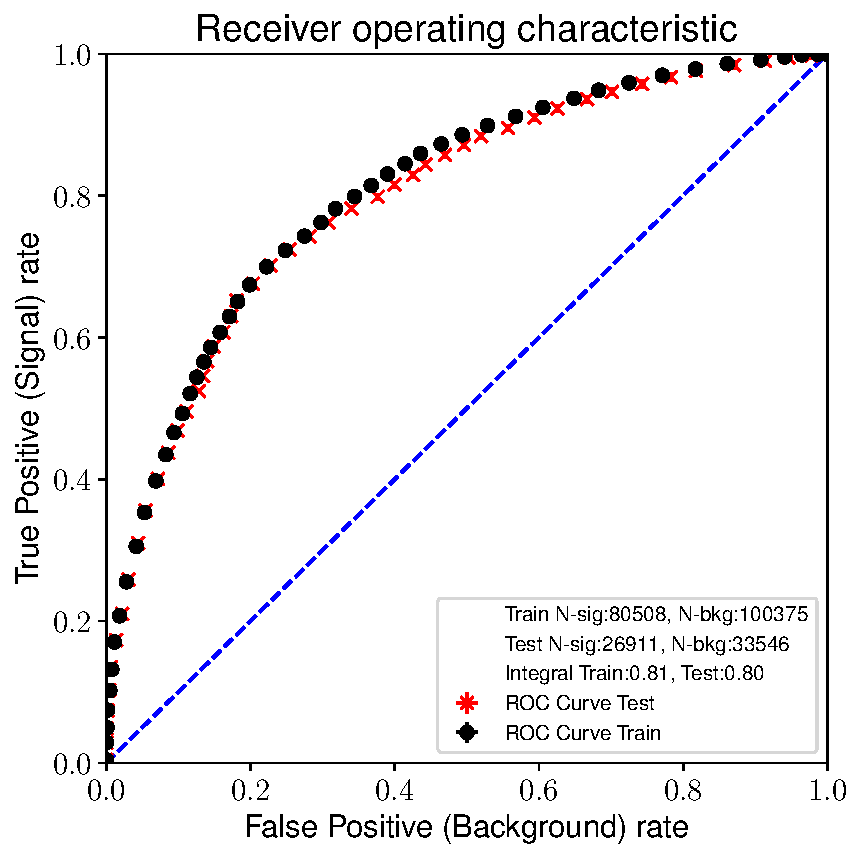
\includegraphics[width=0.48\textwidth]{figures/hmm/bdtHist/roc-3lep-WH-AllBackground-0-depth2-nEst50tag-new-AllBackground.pdf}
  \caption{4 lepton (left) and 3 lepton (right) ROC curves for representative BDT's. Shown in black is the curve for the training set, while red shows the curve for the validation set (labeled test set). Error bars are statistical only. The AUC is labeled on each plot.}
    \label{fig:hmmBdtRoc}
\end{figure}

Figure \ref{fig:hmmBdtScoreLin} shows the BDT discriminant response for different categories of signal and background, scaled the samples cross section and luminosity. The signal/background separation is more apparent in this plot than in those normalized to the physical expectation.


\begin{figure}[htpb]
  \centering
  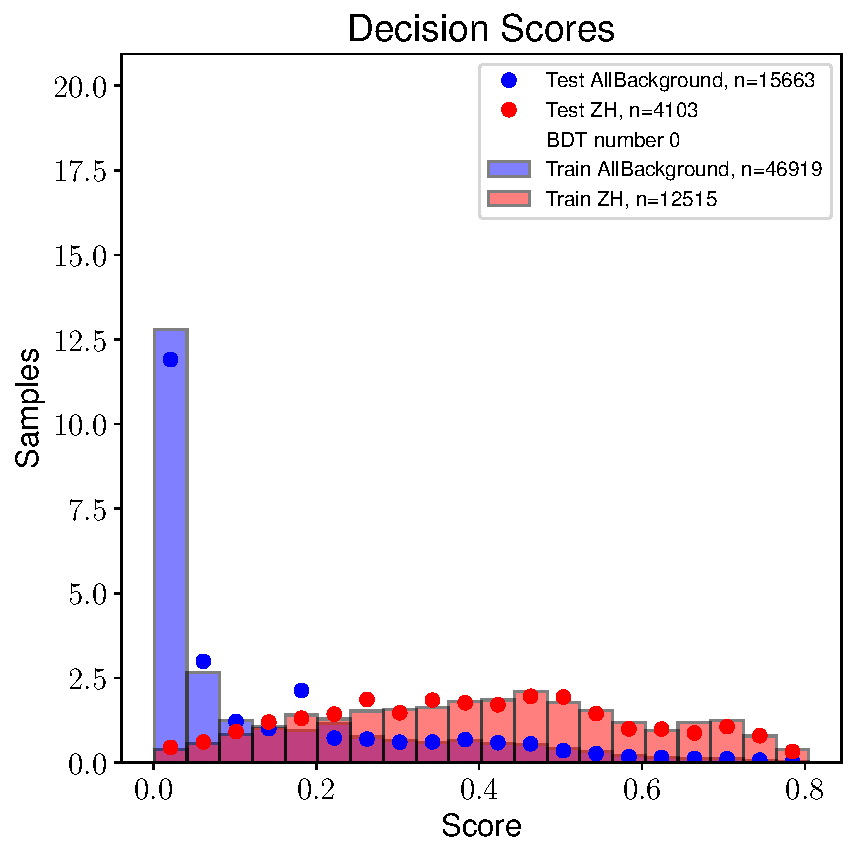
\includegraphics[width=0.48\textwidth]{figures/hmm/bdtHist/bar20-4lep-ZH-AllBackground-0-depth2-nEst80tag-new-AllBackground.pdf}
  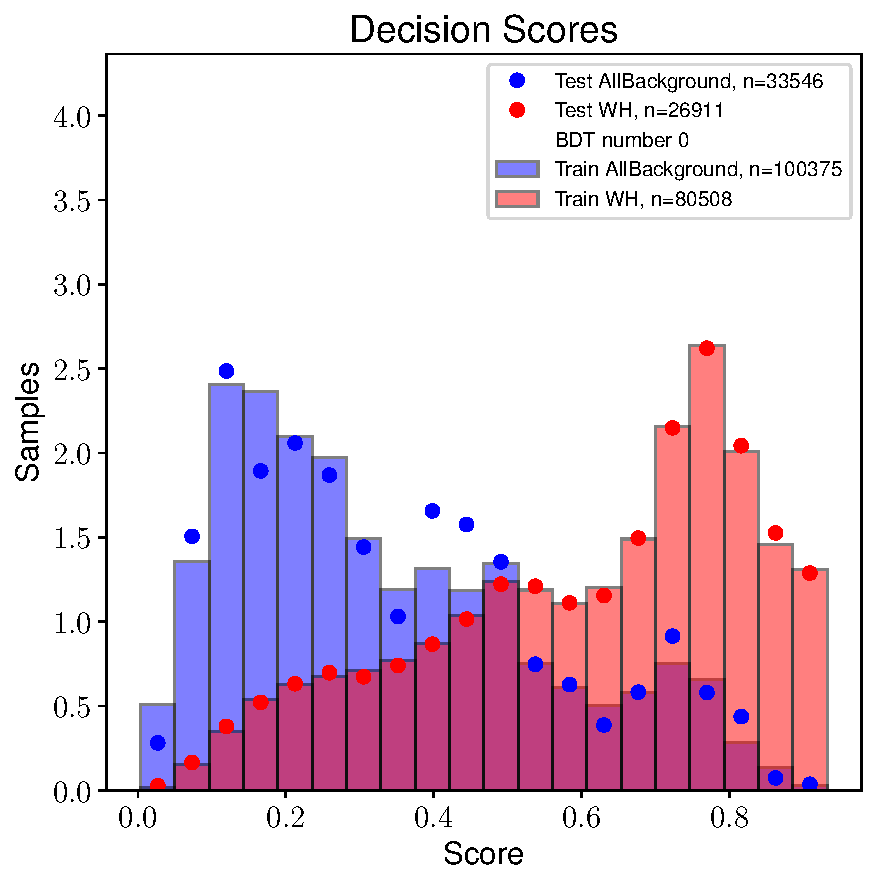
\includegraphics[width=0.48\textwidth]{figures/hmm/bdtHist/bar20-3lep-WH-AllBackground-0-depth2-nEst50tag-new-AllBackground.pdf}
  \caption{4 lepton (left) and 3 lepton (right) distributions of the BDT discriminant, where the signal and background samples share a normalization. The signal distribution is that of the sample used for training, not the full signal MC sample.}
    \label{fig:hmmBdtScoreLin}
\end{figure}

Figure \ref{fig:hmmBdtScore} shows the BDT discriminant response for different categories of signal and background, scaled the samples cross section and luminosity. The composition of the background and signal is more apparent in these plots: primarily the target signal production mechanism is separated. Top backgrounds are particularly well separated owing in part to the high statistics available for these samples.

For 4-lepton case, category ``VH4Lep-High'' is selected by requiring 4-lepton BDT 
score greater than 0.12. 
And for 3-lepton case, two categories ``VH3Lep-High'' and ``VH3Lep-Low'' are selected. The former
is selected by requiring 3-lepton BDT score greater than 0.7,
and the latter is selected by requiring 3-lepton BDT score less than 0.7
but greater than 0.1.
The events failing VH categorization selection are sorted into ggF and
VBF categories as described in Section \ref{sec:hmmCategorization-ggF-VBF}.
 
\begin{figure}[htpb]
  \centering
  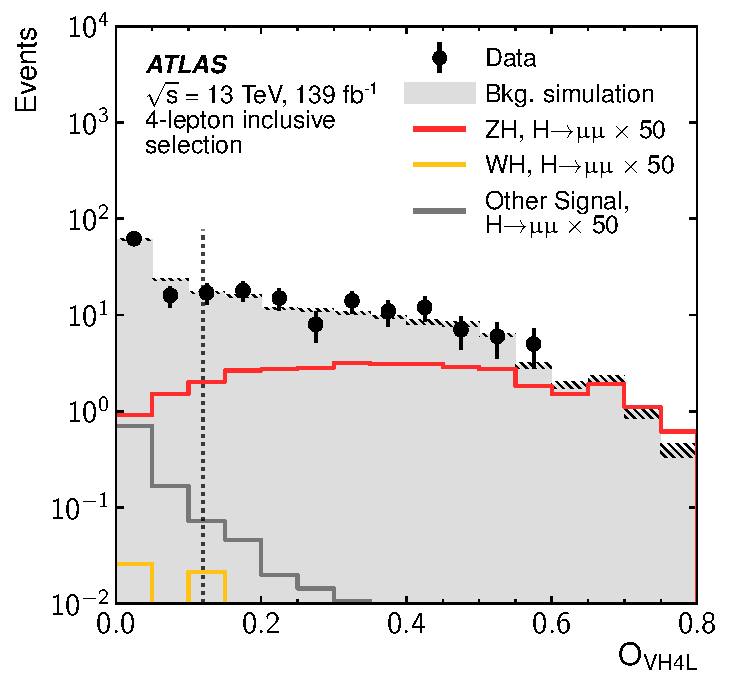
\includegraphics[width=0.48\textwidth]{figures/hmm/public/bdt/histo-4lep-bdtScore.pdf}
  \includegraphics[width=0.48\textwidth]{figures/hmm/public/bdt/histo-3lep-bdtScore.pdf}
  \caption{4-lepton (left) and 3-lepton (right) distributions of the BDT discriminant, using the final test scores. The simulated background is shown in shaded grey, while the signal distributions are drawn as lines in red for ZH and orange for WH. The remaining non-VH production mechanisms (ggF, VBF, and ttH) are combined and plotted as a dark grey line. All the signal histograms have been scaled by a factor of 50 to enhance visibility.\\
  It is clearly observed that the score separates signal to the left and background to the right. Of similar importance is that it specifically isolates the VH signal of interest, and not the other signal productions. For 4-lepton this is the ZH signal and for 3-lepton this is the WH signal. Vertical dotted lines indicate the values that delineate which events belong in which final categories. The full dataset is included as well, which is used to fix the normalization of the background. \\
  Comparing the separation power of the two discriminant, the 3-lepton discriminant is more powerful. This is due in part to the stricter 4-lepton event selection, which is able to remove many more ``easily'' separable background events. The remaining events are more similar topologically to the ZH signal.}
    \label{fig:hmmBdtScore}
\end{figure}

\subsection{Categorization}

The event selection results in two selections: 4-lepton and 3-lepton.
Next, using the BDT discriminant scores, these selections are further divided into sub-categories based on the relative purity of the signal.
The 4-lepton category is divided once into low-purity and high-purity categories.
The 3-lepton category, since the event multiplicity is higher, is divided into low-, medium-, and high-purity categories.

Each event belongs to both a validation dataset and a testing dataset, each of which has an associated discriminant score.
The validation scores are considered when selecting the score thresholds between categories.
The testing scores are used for the final hypothesis test and limit setting.
An optimization scan over various thresholds of the expected significance is performed.
The choice of thresholds made that results in the highest expected significance using the validation scores.
These are specified in Table \ref{tab:hmmBdtCuts}.

\begin{table}[htp]
\begin{center}
\begin{tabular}{l l l l}
\toprule
Category & Discriminant \\
\midrule
4-Lepton High-purity & $O\ge0.12$ \\
4-Lepton Low-purity & $O<0.12$ \\
3-Lepton High-purity & $O\ge0.72$ \\
3-Lepton Middle-purity & $0.10\ge O<0.72$ \\
3-Lepton Low-purity & $O<0.10$ \\
\bottomrule
\end{tabular}
\caption{Category definitions based on the ranges of the discriminant value $O$. The output of the BDT is scaled such that $O\in[0,1]$.}
\label{tab:hmmBdtCuts}
\end{center}
\end{table}

To pick the score thresholds using the testing set, and then perform a hypothesis test in categories defined by that threshold, would lead to a misleading signal and background expectation in those categories.
The choice of threshold would be biased to the statistical fluctuations in the test dataset.
This results in categories biased to contain more simulated signal events and fewer simulated background events than would be expected in the data.
Since analysis on the data includes the signal model based on simulation, such a method is unacceptable.

\begin{figure}[htpb]
  \centering
  \includegraphics[width=0.45\textwidth]{figures/hmm/public/postCut/histo-4lep0-muu.pdf} \\
  \includegraphics[width=0.45\textwidth]{figures/hmm/public/postCut/histo-3lep0-muu.pdf} 
  \includegraphics[width=0.45\textwidth]{figures/hmm/public/postCut/histo-3lep1-muu.pdf} 
  \caption{Distributions of \muu in the 4-lepton (top) and 3-lepton (bottom) categories after a cut on the BDT discriminant.}
    \label{fig:hmmPostcutMassHists}
\end{figure}
\clearpage

The high and middle-purity categories are considered for further analysis, while the low-purity events are only analyzed in the inclusive categories defined before the BDT cut.
The distributions of \muu are shown in Figures \ref{fig:hmmPrecutMassHists} and \ref{fig:hmmPostcutMassHists}.
The former shows the inclusive distribution before further categorization with the BDT discriminant.
The latter shows the distributions in the categories defined in Table \ref{tab:hmmBdtCuts}.
The motivation to use the discriminant becomes apparent in these plots when compared to Figure \ref{fig:hmmPrecutMassHists}.
In both the 4-lepton and 3-lepton high-purity categories, Drell-Yan production has been essentially removed.
The background remaining is primarily from diboson sources.
The purity of the signal selection is also clear in the high-purity categories: the categories select for homogeneous ZH or WH depending on their target.


\section{Background Modeling}\label{sec:hmmBkg}

The results of this analysis are based on a comparison between signal and background hypotheses.
The simulated background distributions provide a powerful tool to understand composition and kinematics of the backgrounds in each category.  
These also provide a possible definition of a background hypothesis, but this definition imports a deal of theoretical assumptions.
Instead, an analytic background is developed from the data by fitting a functional form to the observation.

The Figures \ref{fig:hmmPrecutMassHists} and \ref{fig:hmmPostcutMassHists} show the \muu shapes of the simulated background distributions in the pre-cut and post-cut categories respectively.
In all cases, the background is described by a steeply falling \muu distribution with substantial contributions from \Z processes.
This motivates the inclusion of a Breit-Wigner shape in the functional form with the parameters of the \Z boson.
It is also important for the form to be flexible enough to describe the underlying background distribution, without being flexible enough to describe the statistical fluctuations of the observed dataset.
This motivates the inclusion of an exponential term that introduces only one flexible parameter.
The function chosen is defined in Equation \ref{eqn:hmmBkgFunc}. 
\begin{equation}\begin{split}\label{eqn:hmmBkgFunc}
    f_\text{B}(\muu) = (1-a)\times [f_{\text{BW},Z}\otimes\text{Gaus}()]+a\times\exp{b\times\frac{\muu-110\text{ GeV}}{160\text{ GeV}}}
\end{split}\end{equation} 
Here, \muu is the invariant-mass of the Higgs candidate dimuon, in GeV.
The Breit-Wigner function, $f_{\text{BW},Z}$, uses the \Z mass $m_\text{BW}=91.2$~GeV and width $\Gamma_\text{BW}=2.49$~GeV.
It is convolved with a Gaussian  the product of which is a Voigtian shape.
The Gaussian helps describe detector resolution effects, and is centered at \muu with a width 2~GeV.
Two parameters are left to be determined by their agreement to the data.
The first, $a\in[0,1]$, represents the fraction of the background made of Breit-Wigner compared to the exponential term.
The second, $b$, determines the decent of the exponential term.
Equation \ref{eqn:hmmBkgFunc} is used to define a probability density function (PDF) over \mll from which observed events may have been sampled. 
When it is used to model the dataset, PDF is normalized to number of events in the dataset, using a coefficient.
Since this coefficient is a function of $a$ and $b$, and it does not impact the shape of the distribution, it is not discussed.

The procedure to determine the free parameters is referred to as \emph{fitting} the functional form to the observed data.
The \code{minuit} algorithm is used to adjust the free parameters in order to maximize the likelihood that the observed data could be generated by the PDF.
This is performed in each category, and the resulting parameters are given in Table \ref{tab:hmmBkgFitParams}.

\begin{table}[htp]
\begin{center}
\begin{tabular}{l r r r r r r}
\toprule
Category & $a$ & $b$ \\
\midrule
3-lepton & 0.96$\pm$0.13 & -5.08$\pm$0.61 \\
4-lepton & 1.00$\pm$1.00 & -5.75$\pm$1.17 \\
\midrule
4-lepton High Purity & 0.36$\pm$0.66 & -4.53$\pm$15.06 \\
3-lepton High Purity & 1.00$\pm$0.15 & -6.13$\pm$1.01 \\
3-lepton Low Purity  & 0.95$\pm$0.15 & -4.99$\pm$0.68 \\
\bottomrule
\end{tabular}
\caption{Values of $a$ and $b$ fitted to the data in pre-cut (top) and post-cut (bottom) categories. Uncertainties are the statistical constraint of the fit. In the case of the lower multiplicity 4-lepton categories, the constraints on the parameters are $\sim60\%$ correlated, and one of them could be fixed. However this results in a biased estimate of the signal contribution, described in the following section.}
\label{tab:hmmBkgFitParams}
\end{center}
\end{table}

The numbers Functional form in Equation \ref{eqn:hmmBkgFunc} along with in Table \ref{tab:hmmBkgFitParams} define the background hypotheses in each category.
One prediction of these hypotheses are frequencies of events with invariant-masses $\muu\in[110,160]$~GeV.
This is derived from the PDF.
Another prediction is the number of events invariant-masses $\muu\in[120,130]$~GeV
This is derived from the PDF, normalized to the number of observed events in the \emph{sideband} invariant-mass regions $[110,120]$~GeV and $[130,160]$~GeV.

\section{Signal Modeling}\label{sec:hmmSig}

This section describes the signal contribution to the various categories defined in Section \ref{sec:hmmBdt}.
The expected signal contribution in each category is modeled in the \muu distribution with the with the simulated datasets described in Section \ref{sec:hmmSim}.
As the production mechanism is essentially indistinguishable in terms of signal shape, no further effort is made to separate VH events from ggF, VBF, or ttH events.
From this point, the ensemble of production mechanisms is combined and referred to as \emph{signal}.

An empirical functional form is used to parameterize the shape of the signal distribution.
The shape is determined almost entirely by the \pt resolution for muons since the natural width of the Higgs decay is too small to resolve.
As such, a reasonable choice of function is the double sided Crystal Ball (CB) given in Equation \ref{eq:hmmSignal}.
\begin{equation}\label{eq:hmmSignal}
  f_\text{S}(m_{\mu\mu}) =
  \begin{cases}
  \text{CB}_\text{high}(\alpha_\text{high},n_\text{high},\sigma,\bar{x}) & \text{for }m_{\mu\mu}>\bar{x}\\
  \text{CB}_\text{low}(\alpha_\text{low},n_\text{low},\sigma,\bar{x}) & \text{for }m_{\mu\mu}<=\bar{x}\\
  \end{cases}
\end{equation}
Here, $\alpha_\text{low}$ and $\alpha_\text{high}$ values are the cross-over value for the high and low CB functions.
The other parameters are the shared mean and width of the CB functions, $\bar{x}$ and $\sigma$,
while $n_\text{low}$ and $n_\text{high}$ are the powers for the power-law tails of the high and low CB functions.
The CB function itself is defined in Equation \ref{eqn:hmmCb}.
\begin{equation}\label{eqn:hmmCb}
    \text{CB}(x,\alpha,n,\bar{x},\sigma) = 
    \begin{cases}
        \exp{-\frac{(x-\bar{x})^2}{2\sigma^2}} & \text{for }\frac{(x-\bar{x})}{2\sigma}>-\alpha \\
        \left(\frac{n}{|\alpha|}\right)^n \exp{-\frac{|\alpha|}{2}} \left(\frac{n}{|\alpha|}-|\alpha|\right)^{-n} & \text{otherwise}\\
    \end{cases}
\end{equation}
The CB function is normalized when treated as a PDF.
In the signal model, the normalization is scaled to match the expected number of signal events.

The following diagrams in Figures \ref{fig:hmmSignalFitPreCut} and \ref{fig:hmmSignalFitPostCut} show fits of the signal model to the simulated distribution, both before and after categorization with the BDT score.
The corresponding fitted values of signal model parameters parameters are listed in Tables \ref{tab:hmmSignalFitPreCut} and \ref{tab:hmmSignalFitPostCut}.

\begin{figure}[htpb]
  \centering
  \includegraphics[width=0.48\textwidth]{figures/hmm/signalFits/sigfit-cat3lep-TotalWeight.pdf}
  \includegraphics[width=0.48\textwidth]{figures/hmm/signalFits/sigfit-cat4lep-TotalWeight.pdf}
  \caption{Fits of the signal model to the MC signal for the pre-cut distributions. Left is 3-lepton and right is 4-lepton. The blue line shows the fitted signal function, while the black dots show the MC with statistical errors. The plots also display the fitted parameter values, which are also available in the tables in this section.}
    \label{fig:hmmSignalFitPreCut}
\end{figure}

\begin{figure}[htpb]
  \centering
  \includegraphics[width=0.48\textwidth]{figures/hmm/signalFits/sigfit-cat3lep0-TotalWeight.pdf}
  \includegraphics[width=0.48\textwidth]{figures/hmm/signalFits/sigfit-cat4lep0-TotalWeight.pdf}
  \includegraphics[width=0.48\textwidth]{figures/hmm/signalFits/sigfit-cat3lep1-TotalWeight.pdf}
  \includegraphics[width=0.48\textwidth]{figures/hmm/signalFits/sigfit-cat4lep1-TotalWeight.pdf}
  \caption{Fits of the signal model to the MC signal for the post-cut categories. Top left is the 3-lepton high purity, top right is the 4-lepton high purity. Bottom left is the 3-lepton low purity, top right is the 4-lepton low purity. The blue line shows the fitted signal function, while the black dots show the MC with statistical errors. The plots also display the fitted parameter values, which are also available in the tables in this section.}
    \label{fig:hmmSignalFitPostCut}
\end{figure}

\begin{table}[htbp]
 \begin{center}
\begin{tabular}{l r r r r r}\toprule
Parameter & 4-lepton & 3-lepton \\
\midrule
$\alpha_\text{low}$ & 1.1158 & 1.3261 \\
$n_\text{high}$ & 15.6510 & 26.9325 \\
$\bar{x}$ & 124.4918 & 124.4823 \\
$\alpha_\text{high}$ & 1.4322 & 1.4837 \\
$\sigma$ & 2.7966 & 2.9170 \\
$n_\text{low}$ & 4.5983 & 2.6715 \\
\bottomrule\end{tabular}
 \end{center}
 \caption{Parameters of the signal model for the pre-cut categories.}
\label{tab:hmmSignalFitPreCut}
\end{table}

\begin{table}[htbp]
 \begin{center}
\begin{tabular}{l r r r r r}\toprule
Parameter & 4-lepton HP & 4-lepton LP & 3-lepton LP & 3-lepton HP \\
\midrule
$\alpha_\text{low}$ & 1.1588 & 0.8089 & 1.3606 & 1.3359 \\
$n_\text{high}$ & 13.6813 & 9.8994 & 23.9236 & 58.4665 \\
$\bar{x}$ & 124.4409 & 124.7816 & 124.4572 & 124.5061 \\
$\alpha_\text{high}$ & 1.5154 & 1.1011 & 1.5019 & 1.4111 \\
$\sigma$ & 2.8480 & 2.3540 & 2.8822 & 2.9212 \\
$n_\text{low}$ & 4.9436 & 4.1925 & 2.0431 & 2.9402 \\
\bottomrule\end{tabular}
 \end{center}
 \caption{Parameters of the signal model for the post-cut categories.}
\label{tab:hmmSignalFitPostCut}
\end{table}

\subsection{Signal+Background Model}

It is helpful to define the predictions of various ``signal+background'' (S+B) hypotheses.
This combines the signal prediction from Equation \ref{eq:hmmSignal} with the background prediction in Equation \ref{eqn:hmmBkgFunc}.
The Standard Model predicts a particular signal multiplicity, $N_{SM}$.
The relative amplitude of the signal compared to the prediction of the Standard Model is defined as the \emph{signal strength}, \mus.
A range of S+B hypotheses are possible, labeled by the signal strength.
For example, \mus=1 describes hypothesis with the Standard Model signal strength, while \mus=0 describes a ``background-only'' (B) hypothesis.

The S+B hypothesis predicts the relative frequency of events as a function of \muu.
It is defined in Equation \ref{eqn:hmmSbFunc} as the sum of the normalized signal shape PDF $f_\text{S}(\muu)$, and the normalized background PDF $f_\text{B}(\muu)$.
\begin{equation}\begin{split}\label{eqn:hmmSbFunc}
f_\text{S+B}(\muu) = N_\text{S}\times f_\text{S}(\muu) + N_\text{B}\times f_\text{B}(\muu)
\end{split}\end{equation} 
There are three free parameters in Equation \ref{eqn:hmmSbFunc}: the shape parameters $a$ and $b$ that describe the background, and $N_\text{S}\equiv\mus\times N_{SM}$ where \mus is free.
Each of these may be adjusted by \code{minuit} in order to fit the data distribution in each category.
The overall normalization of the function, when treated as a PDF, is normalized as was the case with the background-only function.

In the case that a strong signal is not observed in the data, it is still possible to consider which S+B hypotheses are compatible and incompatible with the observation.
In this case, some set of hypotheses, are considered excluded to a particular confidence level.
To this end, a S+B hypothesis is defined by a fixed \mus, and free parameters $a$ and $b$.




\section{Statistical Analysis}\label{sec:hmmStat}
\section{Results}\label{sec:hmmResults}

